%%%%%%%%%%%%%%%%%%%%%%%%%%%%%%%%%%%%%%%%%%%%%%%%%%%%%%%%%%%%%%%%%%%%%%%%%%%%%%%%
%%  Sample document for preparing papers to  "SPIIRAS_Proceedings"
%%  charset=utf-8
%%%%%%%%%%%%%%%%%%%%%%%%%%%%%%%%%%%%%%%%%%%%%%%%%%%%%%%%%%%%%%%%%%%%%%%%%%%%%%%%

\documentclass[10pt]{SPIIRAS_Proceedings}
\pdfpkresolution=600
\pdfcompresslevel=1
\usepackage{float}
\usepackage{array}
\usepackage{graphicx}
\graphicspath{{../figures/}{figures/}{image/}{./}}
\usepackage{amsmath}
\usepackage{amssymb}
\usepackage{url}

\newcolumntype{L}[1]{>{\raggedright\arraybackslash}p{#1}}
\newcolumntype{C}[1]{>{\centering\arraybackslash}p{#1}}
\newcolumntype{R}[1]{>{\raggedleft\arraybackslash}p{#1}}
\renewcommand{\arraystretch}{1.18}
\setlength{\tabcolsep}{3.5pt}

\makeatletter
\setcounter{secnumdepth}{2}
\renewcommand{\thesection}{\arabic{section}}
\renewcommand{\thesubsection}{\arabic{section}.\arabic{subsection}}
\def\@seccntformat#1{\csname the#1\endcsname.\space}
\renewcommand\section{\@startsection{section}{1}{\parindent}%
  {\z@}%
  {-0.5em}%
  {\normalfont\normalsize\bfseries}}
\renewcommand\subsection{\@startsection{subsection}{2}{\parindent}%
  {\z@}%
  {-0.5em}%
  {\normalfont\normalsize\bfseries}}
\makeatother

\begin{document} 

\udk{006.72}
\titleEng{Acamind: An Intelligent Academic Question Answering System Integrating Retrieval-Augmented Generation and Hybrid Search for the Psychology Domain}
\authorsTitleEng{D.T.H. \smallcapsfake{CHI}, L.D. \smallcapsfake{TUAN}, N.C. \smallcapsfake{BINH}, N.V. \smallcapsfake{HUNG}} % \smallcapsfake is needed for a small capitall letters, because the used font doesn't support this feature
\authorsEng{Chi D.T.H., Tuan L.D., Binh N.C., Hung N.V.}

\abstractEng{Evidence-Based Practice in clinical psychology requires comparative evaluation across empirical intervention studies. Existing Retrieval-Augmented Generation (RAG) frameworks face two primary algorithmic bottlenecks in this domain: high computational latency from full cross-encoder reranking on CPU hardware and single-document dominance during multi-document synthesis, alongside ingestion noise from scanned PDFs.\par
This paper presents Acamind, a Modular RAG architecture for clinical literature synthesis. Built upon a supporting data infrastructure combining a character-density Scan Circuit Breaker with a hierarchical parent-child index in PostgreSQL, Acamind introduces two methodological contributions: first, a parallel hybrid retrieval pipeline integrating title-boosted pairwise conjunctive-disjunctive full-text search and governed by Dynamic Confident-Skip Reranking (DCSR), which uses Reciprocal Rank Fusion (RRF) rank consensus as an online gate to bypass neural reranking while applying a multi-target Corrective RAG (CRAG) abstention gate; and second, a Multi-Target Decomposition and Quota-Balanced Interleaving synthesis framework paired with explicit document-page header binding and structure-aware multi-chunk disjoint slot extraction.\par
Evaluated across 500 psychology papers (70,825 indexed chunks) and 50 benchmark queries, Acamind achieves a mean warm database retrieval latency of 957.3 ms, a mean end-to-end response time of 4.88 s, and a context relevance of MRR@10 = 0.9833 (Recall@10 = 1.0000). Across the 45 in-scope clinical queries, Acamind answers 44/45 (97.8\%) queries and achieves 0.9667 unconditional human claim faithfulness (0.9886 conditional on answered queries) and 88.9\% unconditional human-verified page citation support (90.9\% conditional), significantly outperforming Naive Dense (37.8\%, $p_{\mathrm{Holm}} = 4.54 \times 10^{-6}$) and BM25 (32.2\%, $p_{\mathrm{Holm}} = 1.89 \times 10^{-6}$). Furthermore, Multi-Target Decomposition raises dual-study retrieval Hit@6 from 60.0\% (9/15) to 100.0\% (15/15, exact McNemar $p = 0.0313$) and achieves 90.0\% (108/120 cells) human-verified accuracy across the 4-attribute clinical comparison matrix.\par
Meanwhile, DCSR bypasses cross-encoder reranking on 31.1\% of in-scope queries (28.0\% of all queries), reducing cold CPU retrieval mean latency by 26.8\% across all 50 queries (30.0\% on in-scope queries) with zero statistically significant ranking loss ($p_{\mathrm{Holm}} = 1.0000$ on MRR@10), while the multi-target CRAG gate refuses 100.0\% of out-of-domain and hard unanswerable prompts with 0.0\% false refusal on in-scope clinical queries.}

\keywordsEng{retrieval-augmented generation, cross-article synthesis, dynamic confident-skip reranking, parallel hybrid search, evidence-based practice, clinical psychology, citation grounding.}

\makeengtitle

\normalsize
\raggedbottom

\section{Introduction.} This section establishes the clinical motivation for automated evidence synthesis in psychology, identifies the core technical bottlenecks of standard Retrieval-Augmented Generation (RAG) pipelines, and summarizes the methodological contributions of Acamind.

\subsection{Context and Motivation.} Evidence-Based Practice (EBP) \cite{sackett1996evidence} is a foundational standard in clinical psychology and psychiatric medicine. Clinical psychologists and healthcare practitioners synthesize, contrast, and integrate empirical findings across clinical trials to formulate diagnostic and psychotherapeutic protocols \cite{moher2009preferred}. The rapid expansion of literature indexed in repositories such as PubMed, PsycINFO, and ScienceDirect creates clinical information overload. Synthesizing intervention studies, cohort sizes, standardized assessment scales (such as BDI-II \cite{beck1996manual}, PHQ-9 \cite{kroenke2001phq}, GAD-7 \cite{spitzer2006brief}, and DASS-21 \cite{lovibond1995structure}), and statistical effect sizes \cite{cohen1988statistical} requires time-consuming manual cross-referencing by domain specialists.

Retrieval-Augmented Generation (RAG) \cite{lewis2020retrieval} addresses this challenge by coupling external database retrieval with Large Language Models (LLMs) to ground generated responses in source documents. However, standard RAG frameworks developed for general question answering face methodological and engineering limitations when applied to clinical literature synthesis \cite{gao2024modular}.

\subsection{Technical Challenges of Traditional RAG in Clinical Literature.} Our empirical evaluation on a corpus of 500 clinical psychology research papers (12,414 pages) and a 50-query clinical benchmark identified two core algorithmic bottlenecks alongside an ingestion hygiene prerequisite:

\textbf{(1) Core Challenge 1: Computational Latency of Full Cross-Encoder Reranking.} Clinical queries require matching both conceptual semantics and exact clinical nomenclature. Hybrid retrieval combining dense vectors \cite{wang2022text} and sparse lexical search \cite{robertson2009probabilistic} fused via Reciprocal Rank Fusion (RRF) \cite{cormack2009reciprocal} improves candidate recall. However, as measured in our CPU retrieval benchmark, passing every fused candidate pool ($K_{\mathrm{rerank}} = 16$ candidates) through a neural cross-encoder \cite{chen2024bge,xiao2023cpack,baai2024bgererankerv2m3} incurs a mean cold latency of 21,297.4~ms (21.30~s) per query, adding 20,183.5~ms of neural inference overhead over raw RRF fusion (1,113.9~ms). When the top candidate chunk already exhibits strong rank consensus across dense and sparse modalities, running full cross-encoder inference across the entire candidate pool adds avoidable computational delay \cite{gao2024modular}.

\textbf{(2) Core Challenge 2: Single-Document Dominance and Score Dilution in Multi-Document Synthesis.} Standard RAG pipelines \cite{izacard2021leveraging,liu2023llamaindex} index literature as a flat collection of text chunks and execute a single combined query pass. When a researcher submits a multi-study comparison or literature synthesis query \cite{moher2009preferred}---for example, contrasting Cognitive Behavioral Therapy (CBT) and Acceptance and Commitment Therapy (ACT) on BDI-II \cite{beck1996manual} outcomes and effect sizes \cite{cohen1988statistical}, or synthesizing three distinct empirical studies---single-pass retrieval suffers from two compounding failures: (a) passages from one paper with higher lexical density monopolize the top-$K$ slots \cite{izacard2021leveraging,gao2024modular}, and (b) evaluating a neural cross-encoder between a multi-paper query and any single-paper chunk depresses relevance logits (since each chunk covers only $1/M$ of the query's targets), triggering false abstentions at pre-LLM confidence gates. In our ablation of 15 two-study comparative queries without sub-query decomposition, single-pass retrieval recovered chunks from both target studies within the top-6 window on only 60.0\% (9/15) of queries, whereas single-modality baselines answered 0\% to 13.3\% of comparative and synthesis prompts.

\textbf{(3) System Prerequisite: Ingestion Noise from Scanned PDFs.} Academic psychology archives contain both digital-born PDFs and legacy scanned reports with missing text layers or corrupted font tables \cite{lo2020s2orc}. Standard ingestion pipelines \cite{gao2023retrieval} extract text without auditing page-level character density. When scanned pages lack an embedded text layer, naive extractors emit empty or garbled chunks \cite{lo2020s2orc}; in our audit of the 500 clinical PDFs, 1 legacy scanned PDF (3 pages) yielded 0 extractable characters per page. Embedding such degenerate or font-corrupted strings into unit-normalized contrastive vector spaces \cite{wang2022text} produces non-zero vectors that can enter top-$K$ retrieval results and degrade generation grounding \cite{yan2024corrective}, as confirmed by the 66.7\% scan-induced hallucination rate measured when degraded PDFs bypass page-level filtering in our fault-injection stress test.

\subsection{Key Contributions and Paper Organization.} This paper introduces \textbf{Acamind}, a modular RAG architecture for clinical literature synthesis. We focus on two methodological contributions supported by an indexing and data hygiene infrastructure:

\textbf{(1) Dynamic Confident-Skip Reranking (DCSR) and Multi-Target CRAG Gating over Parallel Hybrid Retrieval (Core Contribution 1):} We combine parallel HNSW Cosine and title-boosted pairwise conjunctive-disjunctive GIN Full-Text Search in PostgreSQL \texttt{pgvector} with Reciprocal Rank Fusion (RRF) \cite{cormack2009reciprocal}, and introduce the DCSR heuristic gating rule. DCSR uses RRF rank consensus and top-rank dominance margins ($\Delta_{\mathrm{RRF}}$) to bypass cross-encoder reranking when dual-modality agreement exceeds thresholds calibrated on a disjoint 42-query development set, while applying a multi-target Corrective RAG (CRAG) \cite{yan2024corrective} pre-LLM abstention gate ($\max_{m} S_2(q^{(m)}) \ge \tau_{\min}$) that evaluates target-specific sub-query relevance.

\textbf{(2) Multi-Target Decomposition, Quota-Balanced Interleaving, and Structure-Aware Matrix Synthesis (Core Contribution 2):} We formulate an end-to-end multi-document routing and synthesis workflow \cite{gao2024modular,skarlinski2024language} that decomposes single-study ($M=1$), comparative ($M=2$), and literature synthesis ($M=3$) queries into target-specific sub-queries, interleaves retrieved chunks via round-robin per-study quotas with fuzzy deduplication ($\tau_{\mathrm{dedup}} = 0.85$), binds context chunks using explicit document-page headers (\texttt{[\{Filename.pdf\} - Trang \{Page\}]}), and populates a 4-attribute clinical comparison matrix via structure-aware multi-chunk disjoint slot extraction.

\textbf{(3) Supporting Infrastructure and Empirical Evaluation:} We implement a supporting ingestion pipeline combining a character-density \textit{Scan Circuit Breaker} with a \textit{Dual-Memory (L1/L2) Parent-Child Index} over 500 psychology papers (70,825 validated micro-chunks). Across our 50-query benchmark, Acamind achieves an empirically measured mean warm retrieval latency of 957.3~ms, a mean end-to-end latency of 4.88~s, and $\mathrm{MRR@10} = 0.9833$ ($\mathrm{Recall@10} = 1.0000$). On the 45 in-scope queries, blinded dual-rater human evaluation verifies that Acamind answers 44/45 (97.8\%) queries with an unconditional claim faithfulness of $0.9667$ ($0.9886$ conditional) and an unconditional page citation support of 88.9\% ($90.9\%$ conditional), outperforming Naive Dense (37.8\%) and BM25 (32.2\%). Multi-Target Decomposition raises dual-study retrieval Hit@6 from 60.0\% to 100.0\% ($15/15$, $p = 0.0313$) and achieves 90.0\% ($108/120$ cells) human-verified clinical matrix accuracy, while DCSR skips cross-encoder reranking on 31.1\% of in-scope queries (28.0\% of all 50 queries), reducing cold CPU retrieval mean latency by 26.8\% overall (30.0\% on in-scope queries) while refusing 100.0\% of out-of-domain and hard unanswerable prompts.

The remainder of this paper is organized as follows. Section~2 reviews related work in RAG architectures, hybrid retrieval, and scientific literature synthesis. Section~3 presents the Acamind architecture, supporting indexing infrastructure, and the mathematical formulations of DCSR and Cross-Article Synthesis. Section~4 reports the experimental setup, metric definitions, retrieval and generation benchmarks, statistical tests, ablation studies, and limitations. Section~5 concludes the paper and outlines future work.

\section{Related Work.} This section reviews the evolution of RAG paradigms, hybrid dense-sparse retrieval with neural reranking, and multi-document synthesis systems in scientific literature.

\subsection{Evolution of RAG Architectures.} Retrieval-Augmented Generation systems have evolved across three architectural paradigms \cite{gao2023retrieval}, as compared in Table~\ref{tab:rag_comparison}:

\textbf{(1) Naive RAG:} Implements a sequential \textit{Index-Retrieve-Generate} pipeline. Documents are split into uniform chunks and encoded into dense vectors, following early open-domain QA designs such as Fusion-in-Decoder (FiD) \cite{izacard2021leveraging}. Retrieval relies on top-$K$ cosine similarity over vector indices, which often struggles with exact clinical acronyms or multi-study comparisons \cite{lewis2020retrieval}.

\textbf{(2) Advanced RAG:} Adds pre-retrieval and post-retrieval stages such as query rewriting, sliding-window chunking, and cross-encoder reranking. These stages improve retrieval precision but increase computational latency \cite{yan2024corrective}.

\textbf{(3) Modular RAG:} Organizes retrieval, routing, and synthesis into reconfigurable modules \cite{gao2024modular}. Acamind follows the Modular RAG design by pairing confidence-gated rerank skipping (DCSR) with sub-query decomposition over a parent-child relational index.

\begin{table}[H]
\centering
\caption{Architectural comparison of RAG paradigms and Acamind}
\label{tab:rag_comparison}
\footnotesize
\begin{tabular}{|L{1.90cm}|L{1.72cm}|L{1.88cm}|L{1.88cm}|L{2.10cm}|}
\hline
\multicolumn{1}{|C{1.90cm}|}{Technical dimension} & \multicolumn{1}{C{1.72cm}|}{Naive RAG} & \multicolumn{1}{C{1.88cm}|}{Advanced RAG} & \multicolumn{1}{C{1.88cm}|}{Modular RAG} & \multicolumn{1}{C{2.10cm}|}{Acamind} \\
\hline
Retrieval strategy & Dense vector only & Sequential hybrid & Dynamic routing & Parallel hybrid RRF \\
\hline
Reranking mechanism & None & Full cross-encoder & Learning-to-rank & Dynamic Confident-Skip \\
\hline
Cross-paper synthesis & Not supported & Fragment concatenation & Sub-query routing & Quota-balanced matrix \\
\hline
Citation grounding & File name only & Text snippet & Segment index & Physical PDF page \\
\hline
Memory hierarchy & Flat single index & Secondary index & Vector and graph & Dual-memory hierarchy \\
\hline
PDF ingestion & Raw text extraction & Basic OCR support & Separate OCR module & Scan Circuit Breaker \\
\hline
\end{tabular}
\end{table}

The architectural differences across columns in Table~\ref{tab:rag_comparison} stem from the design objectives of each paradigm as established in prior literature \cite{gao2023retrieval,gao2024modular}. Naive RAG \cite{lewis2020retrieval,izacard2021leveraging} was designed for single-passage factoid lookup over clean text corpora, which explains why it relies on a single flat vector index with no reranking, no multi-paper synthesis, and only document-level file name attribution. Advanced RAG \cite{gao2023retrieval,yan2024corrective} improves passage ranking by introducing sequential hybrid retrieval and full cross-encoder reranking \cite{chen2024bge}; however, because it reranks every query and draws from a single flat candidate pool, it incurs high CPU latency and allows one lexically dense paper to crowd out other studies during multi-document comparisons. General Modular RAG frameworks \cite{gao2024modular,liu2023llamaindex} support dynamic routing and sub-querying, yet do not enforce per-study retrieval quotas, physical PDF page binding, or optical scan filtering. Acamind (our proposed architecture in the final column) addresses these clinical Evidence-Based Practice requirements \cite{sackett1996evidence,moher2009preferred} by combining parallel hybrid RRF \cite{cormack2009reciprocal} and Dynamic Confident-Skip Reranking (DCSR) to bypass redundant CPU cross-encoder inference, quota-balanced matrix synthesis with physical PDF page citations, and a dual-memory (L1/L2) parent-child index protected by the Scan Circuit Breaker and vision OCR fallback \cite{lo2020s2orc}.

\subsection{Hybrid Retrieval and Semantic Reranking Strategies.} Single-modality retrieval involves a trade-off between semantic generalization and lexical specificity. Dense vector retrieval \cite{wang2022text} captures paraphrased clinical concepts but can miss exact diagnostic codes or assessment scale abbreviations. Sparse lexical retrieval (BM25 \cite{robertson2009probabilistic}) matches exact tokens but fails on synonymous terminology. Fusing dense and sparse rankings via Reciprocal Rank Fusion (RRF) \cite{cormack2009reciprocal} improves recall across both regimes. Standard hybrid pipelines then pass all top-$K$ candidates to a neural cross-encoder \cite{chen2024bge,xiao2023cpack,baai2024bgererankerv2m3}. Acamind reduces this CPU bottleneck by skipping the cross-encoder when RRF rank agreement is already strong.

\subsection{Cross-Document Synthesis in Scientific Literature.} Recent scientific QA frameworks such as PaperQA2 \cite{skarlinski2024language} use multi-agent iterative search and summarization loops. While effective on open-ended literature reviews, multi-step agent loops require multiple LLM calls per query, resulting in long response times. Commercial tools such as Elicit and SciSpace operate as cloud services where full PDFs are uploaded to external servers. Acamind targets local institutional deployments by keeping PDF storage and hybrid indexing in PostgreSQL while transmitting only retrieved text snippets for synthesis.

\section{Proposed Method: Acamind Architecture.} Acamind comprises a supporting data preparation layer---combining optical density auditing and dual-memory parent-child indexing---and two core algorithmic modules: Parallel Hybrid Retrieval with Dynamic Confident-Skip Reranking (DCSR), and Decomposition-Driven Cross-Article Synthesis with page-level citation grounding. An overview of the complete system architecture is given in Figure~\ref{fig:system_architecture}.

\begin{figure}[H]
\centering
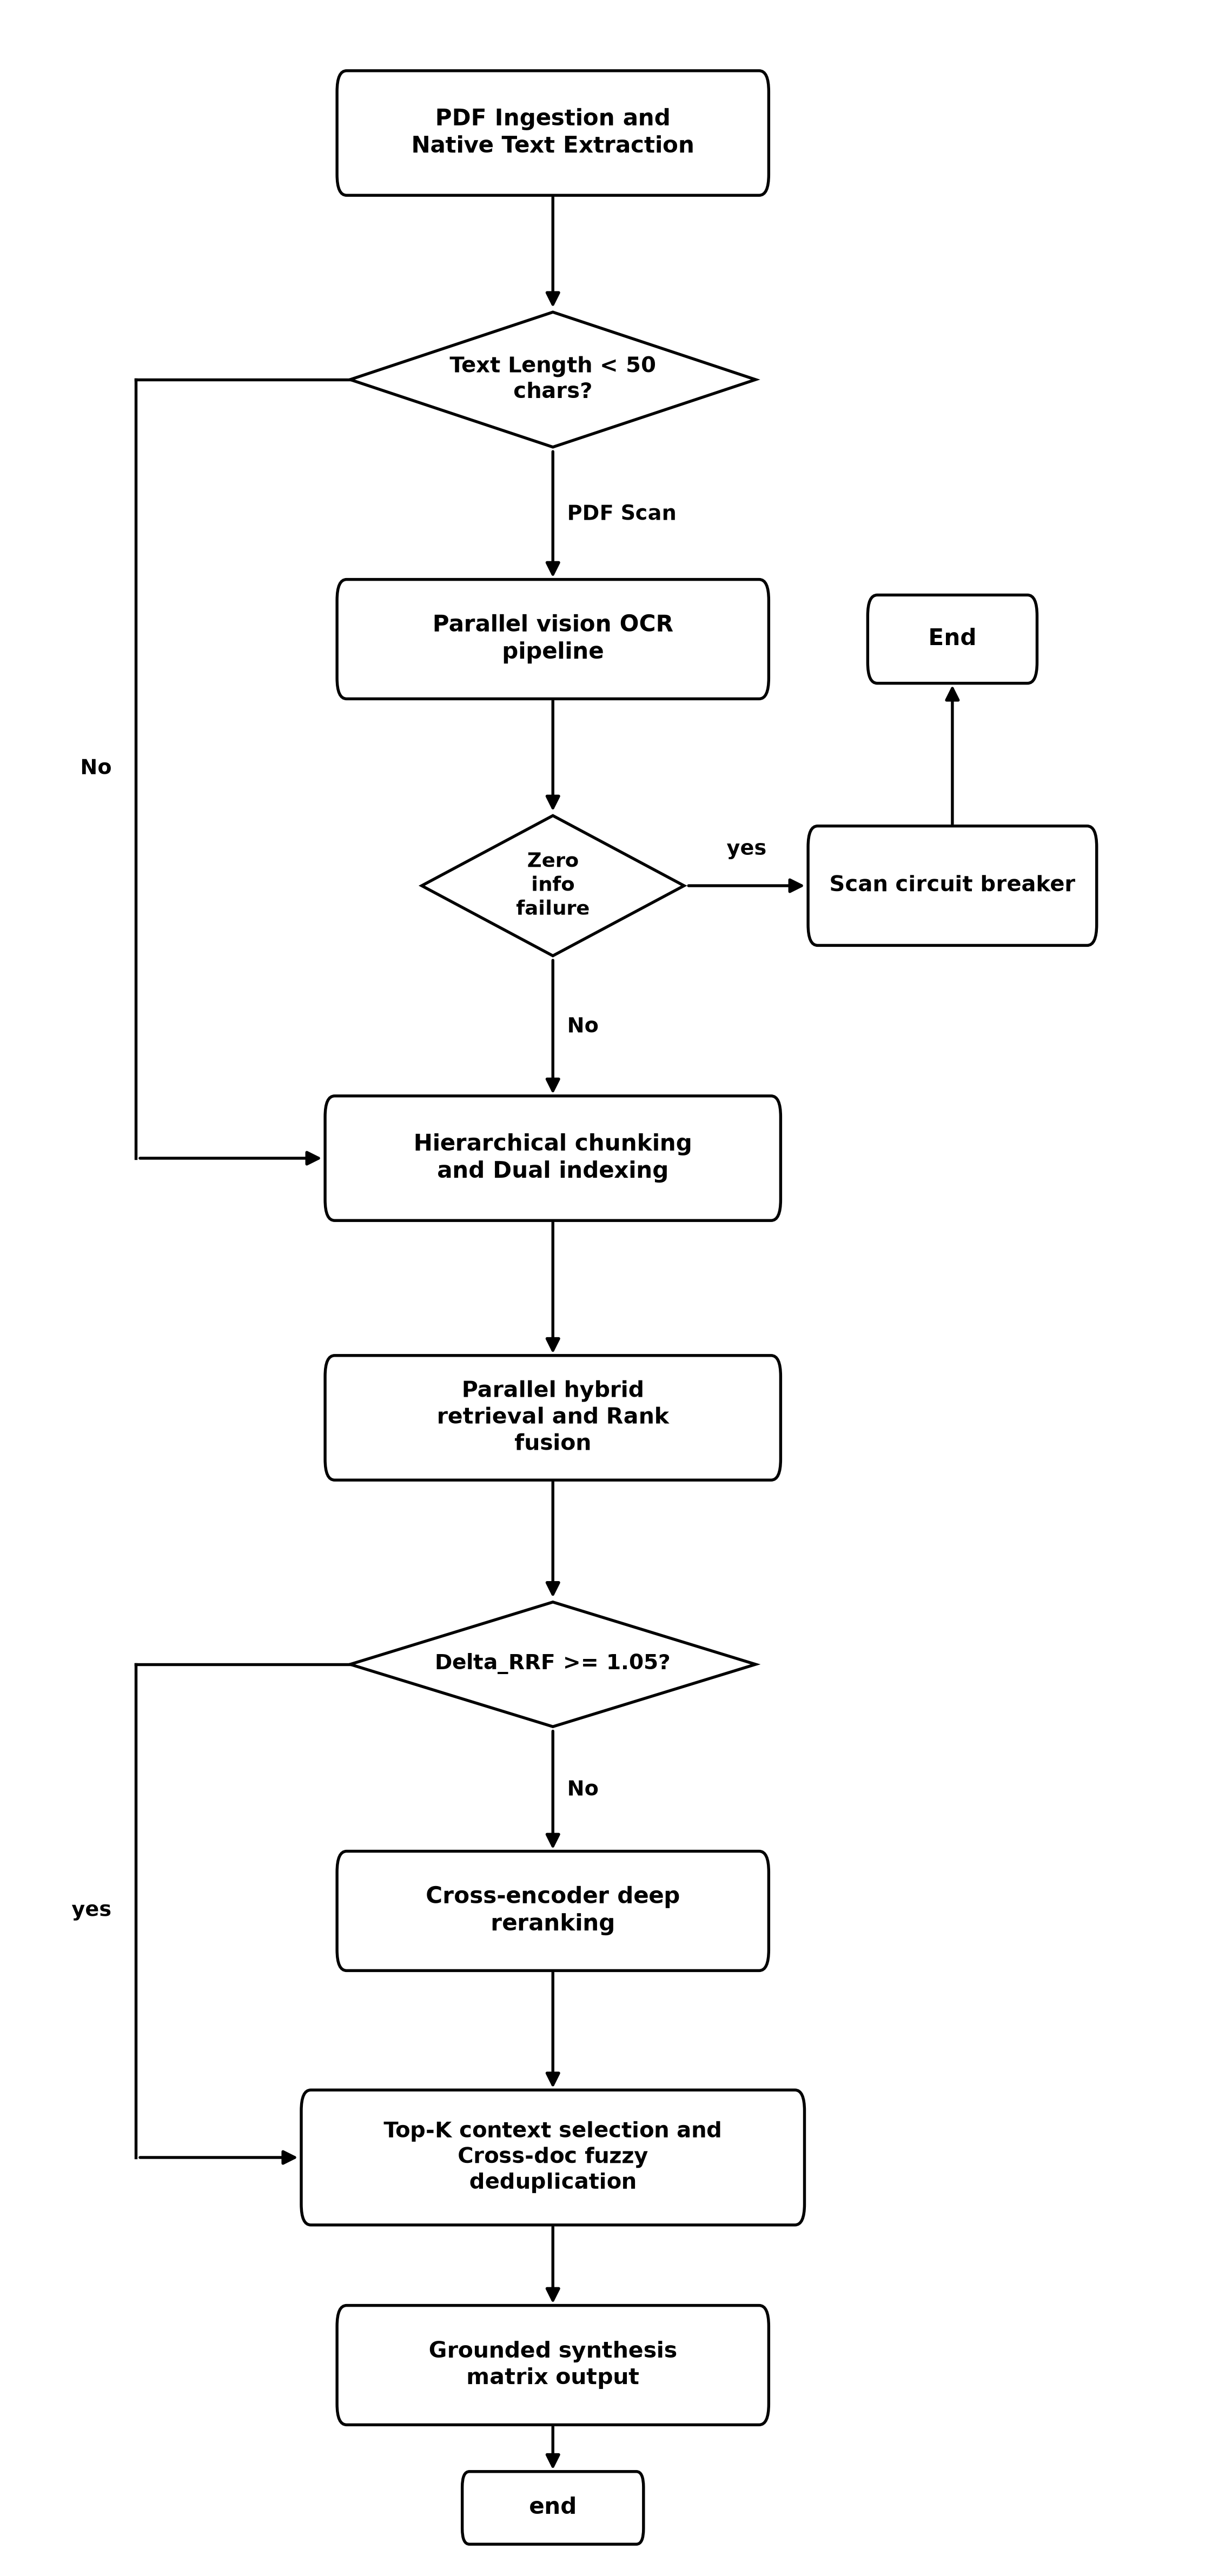
\includegraphics[width=0.58\columnwidth, height=5.8cm, keepaspectratio]{Figure1_System_Architecture.png}
\caption{System architecture of the Acamind Modular RAG framework}
\label{fig:system_architecture}
\end{figure}

Figure~\ref{fig:system_architecture} traces the end-to-end processing flow of Acamind from raw PDF ingestion to grounded response generation. Incoming PDF documents first pass through native text extraction and a character-density check; low-density pages trigger parallel vision OCR or are isolated by the Scan Circuit Breaker if no valid text can be recovered. Validated documents are segmented into the hierarchical L1/L2 dual index in PostgreSQL. At query time, parallel dense and sparse retrieval streams are merged via RRF fusion, evaluated by the calibrated DCSR dominance gate ($\Delta_{\mathrm{RRF}} \ge 1.05$) to decide whether cross-encoder reranking can be bypassed, deduplicated across studies, and synthesized into a page-grounded clinical matrix.

\subsection{Supporting System Infrastructure: Scan Circuit Breaker and Dual-Memory Indexing.} \label{sec:parent_child} Before retrieval and synthesis, the supporting ingestion layer enforces optical text density checks and constructs a two-tier parent-child index, as shown in Figure~\ref{fig:pdf_pipeline}:

\textbf{(1) Optical Integrity Guardrail (Scan Circuit Breaker):} To prevent corrupted or unindexed scanned PDFs from entering the vector store \cite{lo2020s2orc,gao2023retrieval,yan2024corrective}, each incoming document $D$ with page set $P = \{p_1, p_2, \dots, p_{|P|}\}$ and extracted page text $T_p$ undergoes a character density check:

\begin{equation}
C_{\mathrm{density}}(D) = \frac{1}{|P|} \sum_{p \in P} \mathrm{len}(\mathrm{clean}(T_p)),
\label{eq:cdensity}
\end{equation}

\noindent where $\mathrm{clean}(T_p)$ denotes the sanitized text of page $p$ after stripping control characters and Unicode replacement glyphs, and $|P|$ is the total number of pages in document $D$. Equation~(\ref{eq:cdensity}) computes the average density of valid, readable characters per page so the ingestion pipeline can distinguish digital-born clinical articles from unindexed image scans.

Pages with fewer than $\theta_{\mathrm{density}} = 50$ characters are routed to a parallel OCR fallback. The threshold $\theta_{\mathrm{density}} = 50$ characters/page is grounded in our empirical corpus audit of the 500 clinical PDFs, where all 499 digital-born articles exhibited a measured density of at least $1,004.66$ characters/page (with a corpus mean of $3,067.79$ characters/page, since even short title or reference pages exceed $150$ characters), whereas the unindexed scanned PDF yielded $0$ characters/page; furthermore, evaluating page-level enforcement at $\theta_{\mathrm{density}} = 50$ across a 300-PDF fault-injection benchmark (1,200 pages) achieved an F1 score of $1.0000$. If the post-OCR text remains empty ($C_{\mathrm{blank}}(D) = 1$) or falls below $\theta_{\mathrm{density}}$, the Scan Circuit Breaker activates a binary refusal flag:

\begin{equation}
F_{\mathrm{SafeRefusal}}(D) = 
\begin{cases} 
1, & \mathrm{if}\ (C_{\mathrm{blank}}(D) = 1) \lor (C_{\mathrm{density}}(D) < \theta_{\mathrm{density}}), \\
0, & \mathrm{otherwise},
\end{cases}
\label{eq:saferefusal}
\end{equation}

\noindent where $F_{\mathrm{SafeRefusal}}(D) \in \{0, 1\}$ indicates whether document $D$ must be quarantined from indexing. When $F_{\mathrm{SafeRefusal}}(D) = 1$, Equation~(\ref{eq:saferefusal}) halts downstream chunking and embedding immediately, preventing empty or corrupted strings from being projected into unit-normalized vector space \cite{wang2022text}.

\begin{figure}[H]
\centering
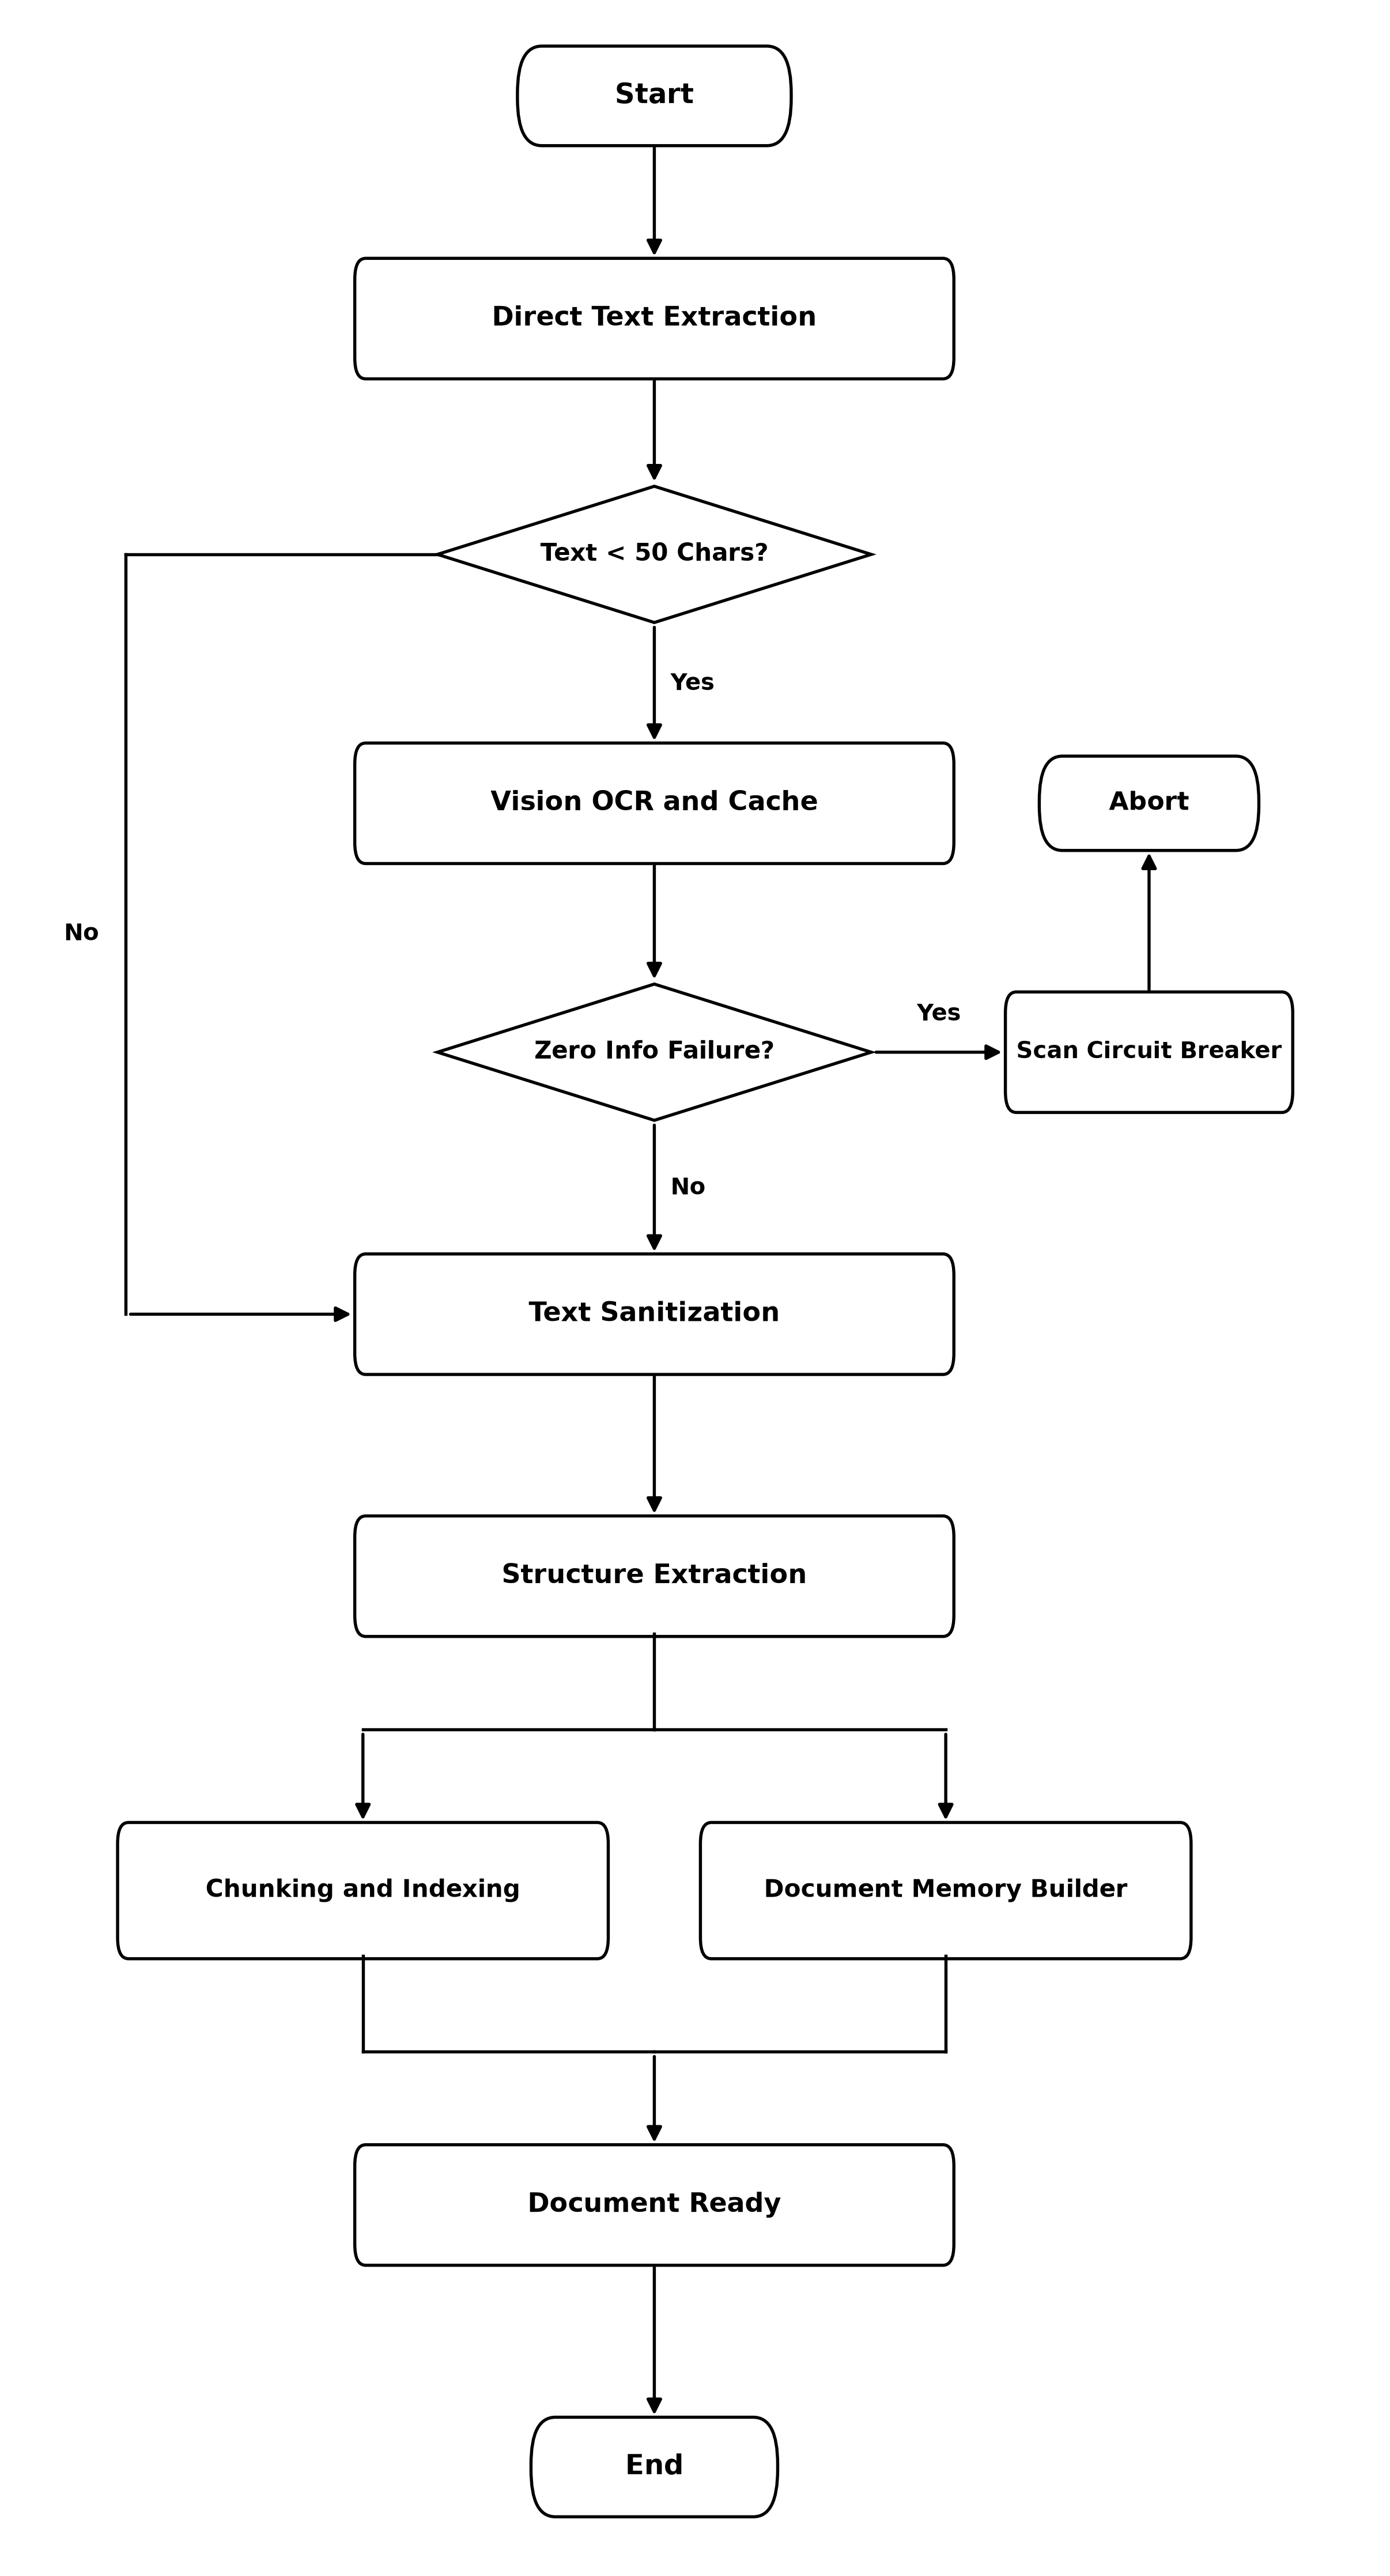
\includegraphics[width=0.58\columnwidth, height=5.5cm, keepaspectratio]{Figure2_PDF_Processing_Pipeline.png}
\caption{Supporting PDF ingestion pipeline with character-density Scan Circuit Breaker}
\label{fig:pdf_pipeline}
\end{figure}

Figure~\ref{fig:pdf_pipeline} illustrates the step-by-step execution of the ingestion pipeline. Each page is first parsed via direct text extraction; if a page contains at least $\theta_{\mathrm{density}} = 50$ characters, it proceeds directly to text sanitization. Pages falling below 50 characters are routed to the vision OCR fallback. If OCR still yields zero readable information, the Scan Circuit Breaker aborts ingestion of the defective file; otherwise, structural metadata and text passages are extracted in parallel by the Chunking Indexer and Document Memory Builder.

\textbf{(2) Dual-Memory Parent-Child Indexing (L1 Fast / L2 Deep):} Validated documents are indexed into two relational tiers in PostgreSQL \cite{izacard2021leveraging,liu2023llamaindex}, illustrated in Figure~\ref{fig:dual_memory}. First, \textit{L1 Fast Memory (Document Tier)} stores document metadata, titles, abstracts, clinical scale tags \cite{beck1996manual,kroenke2001phq,spitzer2006brief,lovibond1995structure}, and summary claims $f$ with confidence $\mathrm{conf}_{\mathrm{LLM}}(f) \in [0, 1]$. Relevance at the L1 tier is scored as:

\begin{equation}
\mathrm{Score}_{\mathrm{L1}}(f) = |T_q \cap T_f| + 5 \cdot \mathbb{I}(q \subseteq f) + \mathrm{conf}_{\mathrm{LLM}}(f),
\label{eq:l1score}
\end{equation}

\noindent where $T_q$ and $T_f$ denote the normalized token sets of query $q$ and summary claim $f$, and $\mathbb{I}(q \subseteq f)$ is an indicator function that equals $1$ when the exact query phrase appears in $f$ (weighted by $5$ to prioritize exact multi-word clinical phrase matches over isolated single-token overlaps). As measured in our L1-only ablation experiment (Table~\ref{tab:ablation_study}), Equation~(\ref{eq:l1score}) scans all 499 document-level summary records in memory in 1.7~ms on average, providing a fast document filter before searching fine-grained passages.

Second, \textit{L2 Deep Memory (Micro-Chunk Tier)} stores fine-grained text chunks segmented using a recursive character splitter configured with an 800-character window and 200-character overlap (producing 70,825 corpus chunks with a measured mean length of 154 words, or $\sim 210$ tokens per chunk), linked to surrounding parent context windows and physical PDF page numbers:

\begin{equation}
\mathrm{Chunk}_{\mathrm{L2}} = \langle \mathrm{ChunkID}, \mathrm{ParentID}, \mathrm{DocTitle}, \mathrm{PageNumber}, \vec{v}_{\mathrm{dense}}, T_{\mathrm{sparse}} \rangle,
\label{eq:chunk_l2}
\end{equation}

\noindent where $\vec{v}_{\mathrm{dense}} \in \mathbb{R}^{768}$ is the L2-normalized dense embedding vector and $T_{\mathrm{sparse}}$ is the PostgreSQL full-text vector representation. Equation~(\ref{eq:chunk_l2}) binds every searchable vector and lexical index entry in PostgreSQL directly to its parent window ($\pm 250$ characters) and physical PDF page coordinate, ensuring that retrieved evidence retains surrounding context and verifiable page provenance.

\begin{figure}[H]
\centering
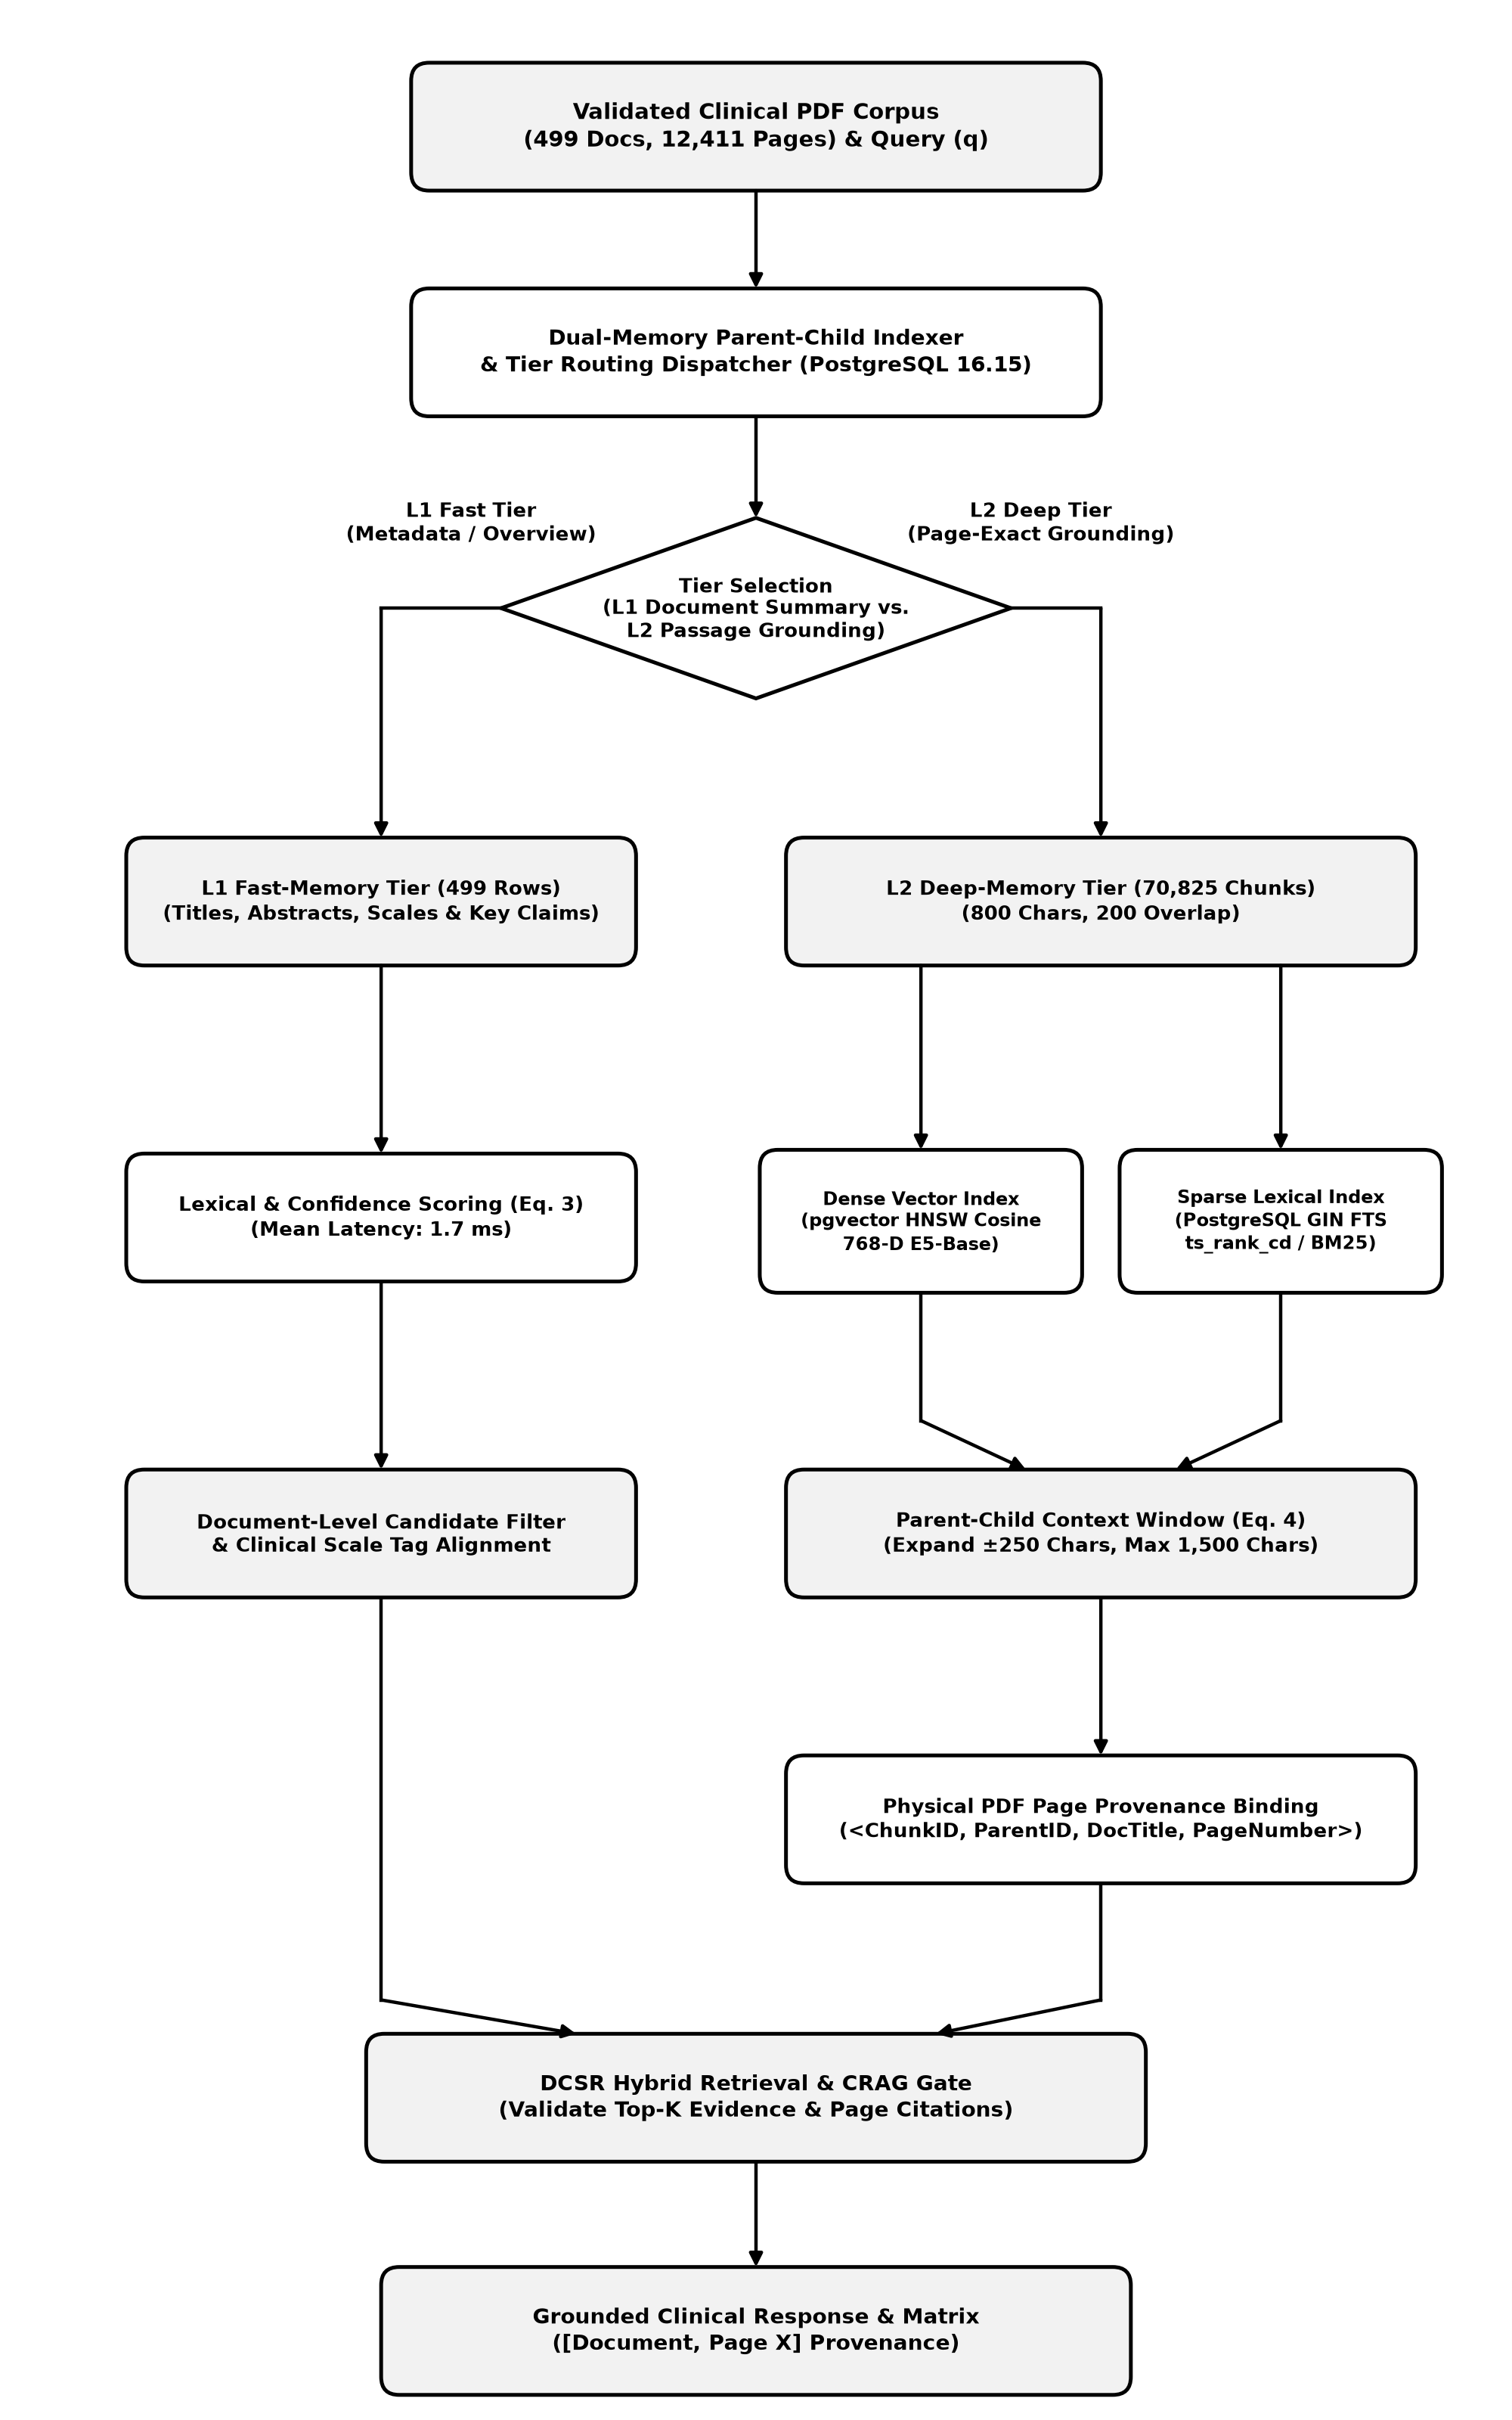
\includegraphics[width=0.60\columnwidth, height=5.5cm, keepaspectratio]{Figure3_Dual_Memory_Knowledge_Graph.png}
\caption{Supporting dual-memory parent-child indexing architecture}
\label{fig:dual_memory}
\end{figure}

Figure~\ref{fig:dual_memory} shows how the Dual-Memory architecture routes queries across the two PostgreSQL storage tiers (L1 Fast Tier and L2 Deep Tier). High-level metadata and overview lookups are handled by the L1 Fast-Memory Tier using Equation~(\ref{eq:l1score}), whereas evidence-based clinical queries requiring exact passage grounding are routed to the L2 Deep-Memory Tier. In the L2 tier, the 70,825 corpus chunks are searched simultaneously via the HNSW dense vector index and the GIN sparse lexical index, expanded with their parent context windows via Equation~(\ref{eq:chunk_l2}), and passed to the DCSR and CRAG verification gates.

\subsection{Core Method I: Parallel Hybrid Retrieval and Dynamic Confident-Skip Reranking (DCSR).} \label{sec:dcsr_method} At the L2 tier, Acamind executes parallel hybrid retrieval followed by the DCSR gating rule, as shown in Figure~\ref{fig:hybrid_retrieval}. Given a query or target sub-query $q$, the pipeline operates across four steps:

\textbf{(1) Dense Semantic Search:} Computes cosine similarity over 768-dimensional embeddings (\texttt{intfloat/multilingual-e5-base} \cite{wang2022text}) via the \texttt{pgvector} HNSW index:

\begin{equation}
\mathrm{Sim}_{\mathrm{dense}}(q, d) = \frac{E(q) \cdot E(d)}{\|E(q)\| \|E(d)\|},
\label{eq:simdense}
\end{equation}

\noindent where $E(q)$ and $E(d)$ denote the 768-dimensional dense embeddings of query $q$ and candidate chunk $d$. Equation~(\ref{eq:simdense}) captures conceptual and paraphrased similarity between the user's clinical question and candidate passages even when exact terminology differs \cite{wang2022text}.

\textbf{(2) Title-Boosted Pairwise Conjunctive-Disjunctive Sparse Lexical Search:} Queries the PostgreSQL GIN Full-Text Search index paired with the BM25 / cover-density lexical relevance formulation \cite{robertson2009probabilistic} ($k_1 = 1.2, b = 0.75$):

\begin{equation}
\mathrm{Score}_{\mathrm{BM25}}(q, d) = \sum_{t \in q} \mathrm{IDF}(t) \cdot \frac{f(t, d)(k_1 + 1)}{f(t, d) + k_1\left(1 - b + b \frac{|d|}{\mathrm{avgdl}}\right)},
\label{eq:scorebm25}
\end{equation}

\noindent where $\mathrm{IDF}(t)$ is the inverse document frequency of query token $t$, $f(t, d)$ is the term frequency of $t$ in chunk $d$, $|d|$ is the chunk length, and $\mathrm{avgdl}$ is the average chunk length across the corpus. In clinical PDF corpora, naive all-AND queries fail when a single query word is paraphrased or truncated at a PDF line break (e.g., \textit{Supporting} split into \textit{Support-}), whereas naive all-OR queries match generic clinical terms across hundreds of unrelated papers. To resolve this, Acamind constructs a pairwise conjunctive-disjunctive tsquery over informative sub-query tokens $\{t_1, \dots, t_L\}$:

\begin{equation}
Q_{\mathrm{pair}}(q) = \bigvee_{i=1}^{L-1} \left(t_i \land t_{i+1}\right) \lor \left(t_1 \land t_L^*\right), \quad \mathrm{Score}_{\mathrm{sparse}}(q, d) = 2.0 \cdot \mathrm{Rank}_{\mathrm{GIN}}(Q_{\mathrm{pair}}, \mathrm{Title}_d) + 1.0 \cdot \mathrm{Rank}_{\mathrm{GIN}}(Q_{\mathrm{pair}}, \mathrm{Text}_d),
\label{eq:titleboost_fts}
\end{equation}

\noindent where $t_L^*$ applies prefix matching (\texttt{:*}) to the trailing token to survive PDF line-break hyphenation, and $\mathrm{Score}_{\mathrm{sparse}}(q, d)$ combines document-title lexical density (weighted by $2.0$) with passage-body lexical density (weighted by $1.0$). Furthermore, an automated reference-section filter strips bibliography and citation-list chunks prior to candidate truncation, preventing reference pages that merely cite a target study from displacing empirical body pages.

\begin{figure}[H]
\centering
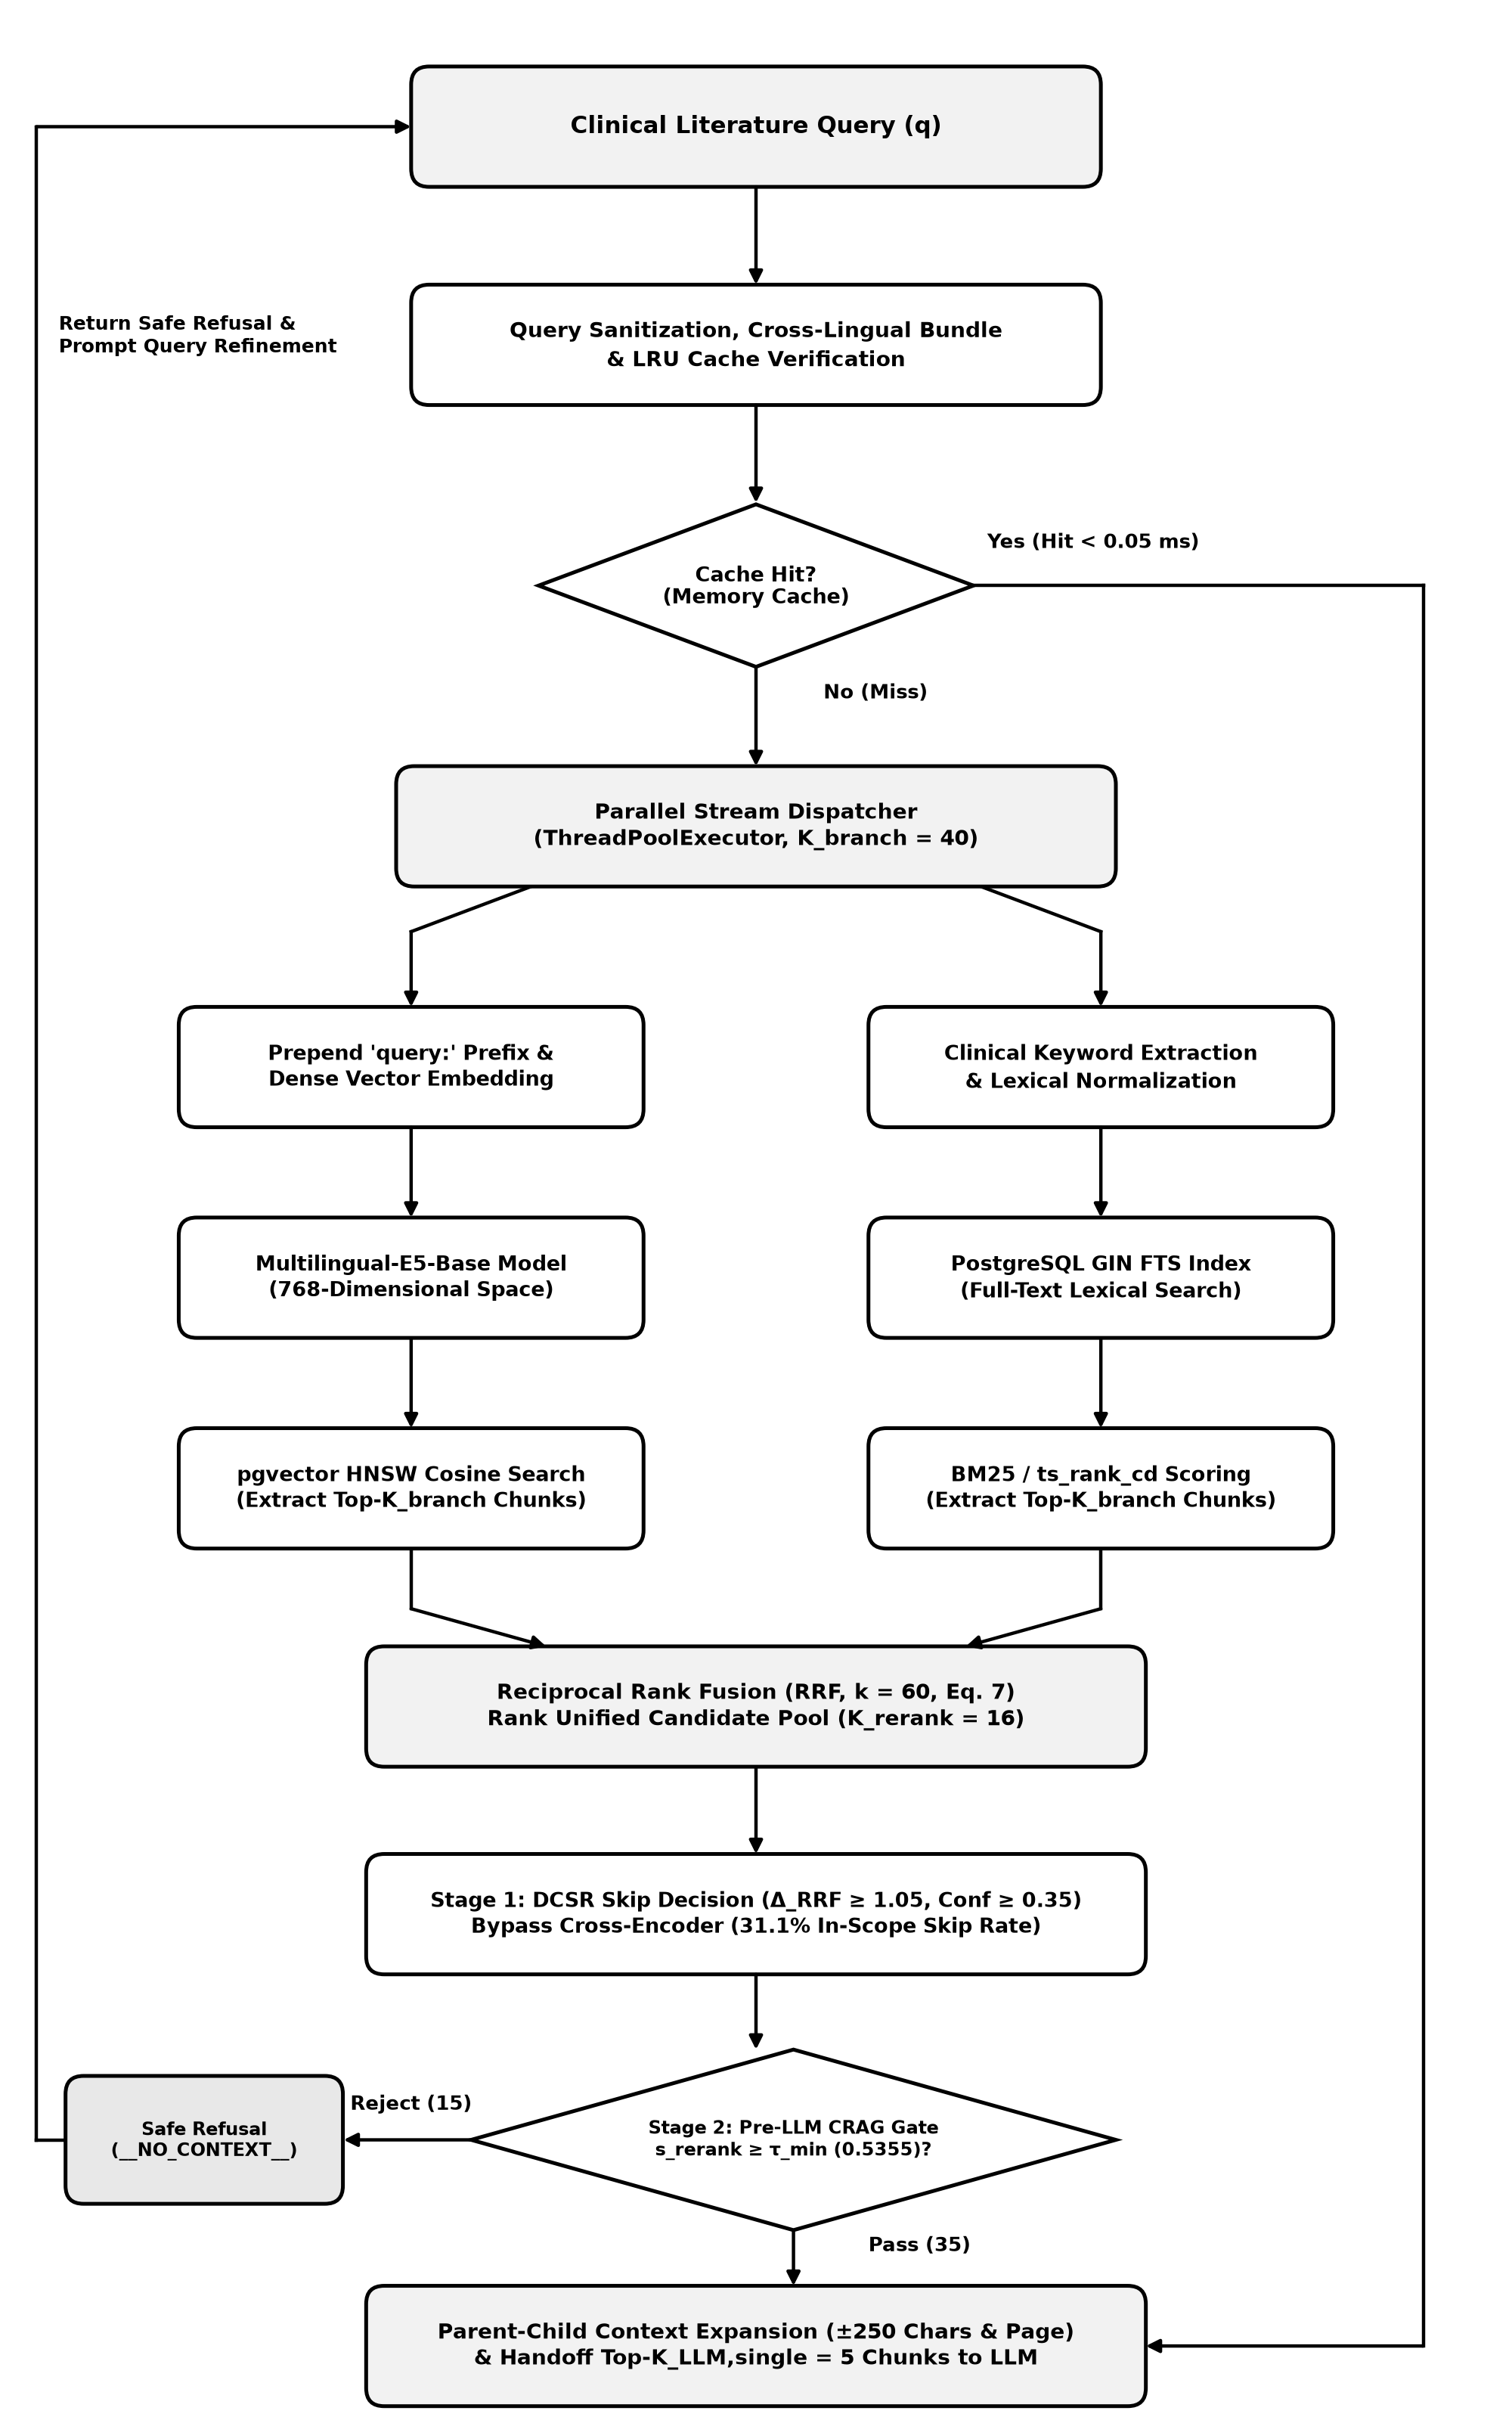
\includegraphics[width=0.58\columnwidth, height=5.8cm, keepaspectratio]{Figure4_Hybrid_Retrieval_Pipeline.png}
\caption{Parallel Hybrid Retrieval workflow combining HNSW Cosine and GIN FTS search}
\label{fig:hybrid_retrieval}
\end{figure}

Figure~\ref{fig:hybrid_retrieval} depicts the execution flow of the parallel hybrid retrieval pipeline. If a query is not found in the in-memory LRU cache, a parallel dispatcher launches the dense HNSW branch and the sparse GIN FTS branch concurrently. Both branches return their top-$K_{\mathrm{branch}}$ candidate lists, which are merged by Reciprocal Rank Fusion (RRF) and evaluated by the two-stage DCSR and CRAG gates before expanding parent context windows for the LLM.

\textbf{(3) Reciprocal Rank Fusion and DCSR Dominance Gating:} The ranked candidate lists from the dense and sparse branches are merged using Reciprocal Rank Fusion (RRF) with the standard smoothing constant $k=60$ established by Cormack et al.~\cite{cormack2009reciprocal}:

\begin{equation}
\mathrm{RRF}(d) = \sum_{m \in \{\mathrm{dense}, \mathrm{sparse}\}} \frac{1}{60 + \mathrm{rank}_m(d)},
\label{eq:rrf}
\end{equation}

\noindent where $\mathrm{rank}_m(d)$ is the 1-based rank of chunk $d$ in retrieval modality $m$. Because dense cosine scores and sparse lexical scores have incompatible numerical scales, Equation~(\ref{eq:rrf}) combines them using rank positions alone \cite{cormack2009reciprocal}, rewarding candidate chunks that rank highly in both retrieval modalities. Table~\ref{tab:k_params} defines the candidate cutoff parameters configured across each stage of the retrieval funnel.

\begin{table}[H]
\centering
\caption{Retrieval and context cutoff parameters across pipeline stages}
\label{tab:k_params}
\footnotesize
\begin{tabular}{|C{1.55cm}|C{1.15cm}|L{2.34cm}|L{4.70cm}|}
\hline
Parameter & Cutoff & \multicolumn{1}{C{2.34cm}|}{Pipeline stage} & \multicolumn{1}{C{4.70cm}|}{Operational role} \\
\hline
$K_{\mathrm{branch}}$ & $40$ & Hybrid SQL search & Candidates fetched per modality from dense and sparse indices \\
\hline
$K_{\mathrm{rerank}}$ & $16$ & Cross-encoder pool & Top RRF-fused candidates evaluated by the cross-encoder \\
\hline
$K_{\mathrm{LLM, single}}$ & $5$ & Single-pass Q\&A & Top parent-expanded chunks passed to the generator \\
\hline
$K_{\mathrm{LLM, decomp}}$ & $6$ & Multi-study synthesis & Total context chunks allocated across compared studies \\
\hline
\end{tabular}
\end{table}

The specific cutoff values in Table~\ref{tab:k_params} are grounded in the empirical latency-recall trade-off measured at each stage of our pipeline. First, $K_{\mathrm{branch}} = 40$ is selected for initial SQL retrieval so that relevant passages ranked at moderate depths (positions $10$--$40$) in one modality can still merge with top-ranked results from the other modality via RRF; as measured in our retrieval benchmark (Table~\ref{tab:retrieval_latency}, Configuration C3), fetching and fusing $40$ candidates per branch takes $957.2$~ms warm ($1,113.9$~ms cold) while raising $\mathrm{MRR@10}$ from $0.5710$ (BM25) and $0.7867$ (Naive Dense) to $0.9574$ ($\mathrm{Recall@10} = 1.0000$). Second, $K_{\mathrm{rerank}} = 16$ is chosen for the cross-encoder pool evaluated by \texttt{BAAI/bge-reranker-v2-m3} \cite{chen2024bge,baai2024bgererankerv2m3} because CPU inference scales linearly with candidate count: in our empirical timing comparison between Configuration C4 (with reranking, $21,297.4$~ms cold) and Configuration C3 (without reranking, $1,113.9$~ms cold), evaluating $16$ candidates adds $20,183.5$~ms of CPU inference ($1,261.5$~ms per candidate chunk), so capping the pool at $16$ bounds worst-case CPU latency at $21.30$~s while raising $\mathrm{MRR@10}$ to $1.0000$ ($0.9833$ under DCSR in Configuration C5). Finally, $K_{\mathrm{LLM, single}} = 5$ provides sufficient parent-expanded context ($\sim 1,300$ characters per chunk) to achieve $90.0\%$ human-verified page citation support and $0.9750$ claim faithfulness on single-study Factual Q\&A (Table~\ref{tab:scenario_evaluation}), whereas $K_{\mathrm{LLM, decomp}} = 6$ is used in multi-study matrix synthesis so that the context window divides evenly into a balanced quota of $k_m = 3$ chunks per target study across $M = 2$ compared studies.

Standard hybrid pipelines pass all $K_{\mathrm{rerank}}$ candidates to a neural cross-encoder (\texttt{BAAI/bge-reranker-v2-m3} \cite{chen2024bge,xiao2023cpack,baai2024bgererankerv2m3}). Acamind instead uses RRF rank consensus as an online gate to skip neural reranking when the top candidate already exhibits clear dominance. Let $c_{(1)}$ and $c_{(2)}$ denote the first- and second-ranked candidates in the fused RRF pool, with $\mathrm{RRF}_{\mathrm{top1}} = \mathrm{RRF}(c_{(1)})$. DCSR computes a scaled confidence score $\mathrm{Conf}(q, \mathcal{C})$ and a top-rank dominance ratio $\Delta_{\mathrm{RRF}}$:

\begin{equation}
\mathrm{Conf}(q, \mathcal{C}) = \min\left(1.0, \; 15.0 \cdot \mathrm{RRF}_{\mathrm{top1}} + \frac{0.5}{1 + e^{-200(\mathrm{RRF}_{\mathrm{top1}} - 0.0165)}}\right),
\label{eq:conf}
\end{equation}

\noindent where $0.0165$ is the mathematical inflection point situated immediately above the maximum RRF score attainable by a chunk retrieved in only a single modality ($\frac{1}{60 + 1} = \frac{1}{61} \approx 0.016393$). By placing the logistic step at $0.0165$, Equation~(\ref{eq:conf}) guarantees that any chunk found by only one retrieval path remains below $\mathrm{Conf} \approx 0.47$, whereas a chunk retrieved near the top of both dense and sparse paths ($\mathrm{RRF}_{\mathrm{top1}} \le \frac{2}{61} \approx 0.032787$) activates the $+0.5$ logistic boost and maps toward $1.0$.

To verify that $c_{(1)}$ also holds a clear lead over the runner-up candidate $c_{(2)}$, DCSR evaluates the dominance ratio:

\begin{equation}
\Delta_{\mathrm{RRF}} = \frac{\mathrm{RRF}(c_{(1)})}{\max(\mathrm{RRF}(c_{(2)}), 10^{-6})},
\label{eq:deltarrf}
\end{equation}

\noindent where $\Delta_{\mathrm{RRF}} \ge 1.0$ measures the relative RRF margin between the first and second candidates. Mathematically, under Equation~(\ref{eq:rrf}) with $k = 60$, if $c_{(1)}$ is retrieved by only one modality, its maximum possible ratio over the next single-modality rank is $\frac{1/61}{1/62} = \frac{62}{61} \approx 1.0164 < 1.05$. Consequently, requiring $\Delta_{\mathrm{RRF}} \ge 1.05$ in Equation~(\ref{eq:deltarrf}) mathematically guarantees both dual-modality retrieval agreement and at least a $5\%$ RRF lead over the second-ranked chunk, preventing premature skipping on tied rank pairs.

\textbf{(4) Two-Stage Execution Order, Multi-Target CRAG Gating, and Empirical Calibration:} All operating thresholds were empirically calibrated on a disjoint 42-query development set ($27$ answerable in-scope queries and $15$ unanswerable queries) and frozen prior to test evaluation (verified via SHA-256 checksum). Specifically, in a 20-point grid search over $(\tau_{\mathrm{conf}}, \tau_{\Delta})$ on the development set, setting $\tau_{\mathrm{conf}} = 0.35$ and $\tau_{\Delta} = 1.05$ bypassed the cross-encoder on $37.0\%$ ($10/27$) of answerable development queries while maintaining $\mathrm{MRR@10} = 1.0000$ and $\mathrm{NDCG@10} = 0.8219$ (zero loss relative to full reranking at $0.8219$). Similarly, via Receiver Operating Characteristic (ROC) analysis on the 42 development queries, the pre-LLM abstention threshold $\tau_{\min} = 0.5355$ on the top cross-encoder relevance score $S_2$ was selected by maximizing Youden's index ($J = 0.8963$), achieving an area under the ROC curve of $\mathrm{AUROC} = 0.9383$ ($\mathrm{TPR} = 96.3\%$, $\mathrm{TNR} = 93.3\%$). For multi-target queries decomposed into $M$ target sub-queries $\{q^{(1)}, \dots, q^{(M)}\}$, evaluating a single cross-encoder pass on the unsplit multi-paper prompt artificially depresses relevance logits because any single chunk covers only one target paper; therefore, the pre-LLM CRAG gate evaluates the maximum per-target relevance score across sub-queries, $\max_{m \in \{1, \dots, M\}} S_2(q^{(m)}) \ge \tau_{\min} = 0.5355$. On the held-out test set, this frozen multi-target gate passes $45/45$ ($100.0\%$) of answerable in-scope queries ($0.0\%$ false gate refusal) while rejecting $5/5$ ($100.0\%$) out-of-domain queries and $10/10$ ($100.0\%$) hard in-domain unanswerable clinical queries ($15/15 = 100.0\%$ combined true refusal). As shown in Figure~\ref{fig:dcsr_flow}, Stage~1 (DCSR Skip Decision) checks immediately after RRF fusion whether $\mathrm{Conf}(q, \mathcal{C}) \ge 0.35$ and $\Delta_{\mathrm{RRF}} \ge 1.05$; when satisfied, cross-encoder reranking is bypassed. Stage~2 (Pre-LLM CRAG Abstention Gate) compares the top candidate score against $\tau_{\min} = 0.5355$ \cite{yan2024corrective} before invoking the LLM, rejecting low-confidence queries with a safe refusal token (\texttt{\_\_NO\_CONTEXT\_\_}).

\begin{figure}[H]
\centering
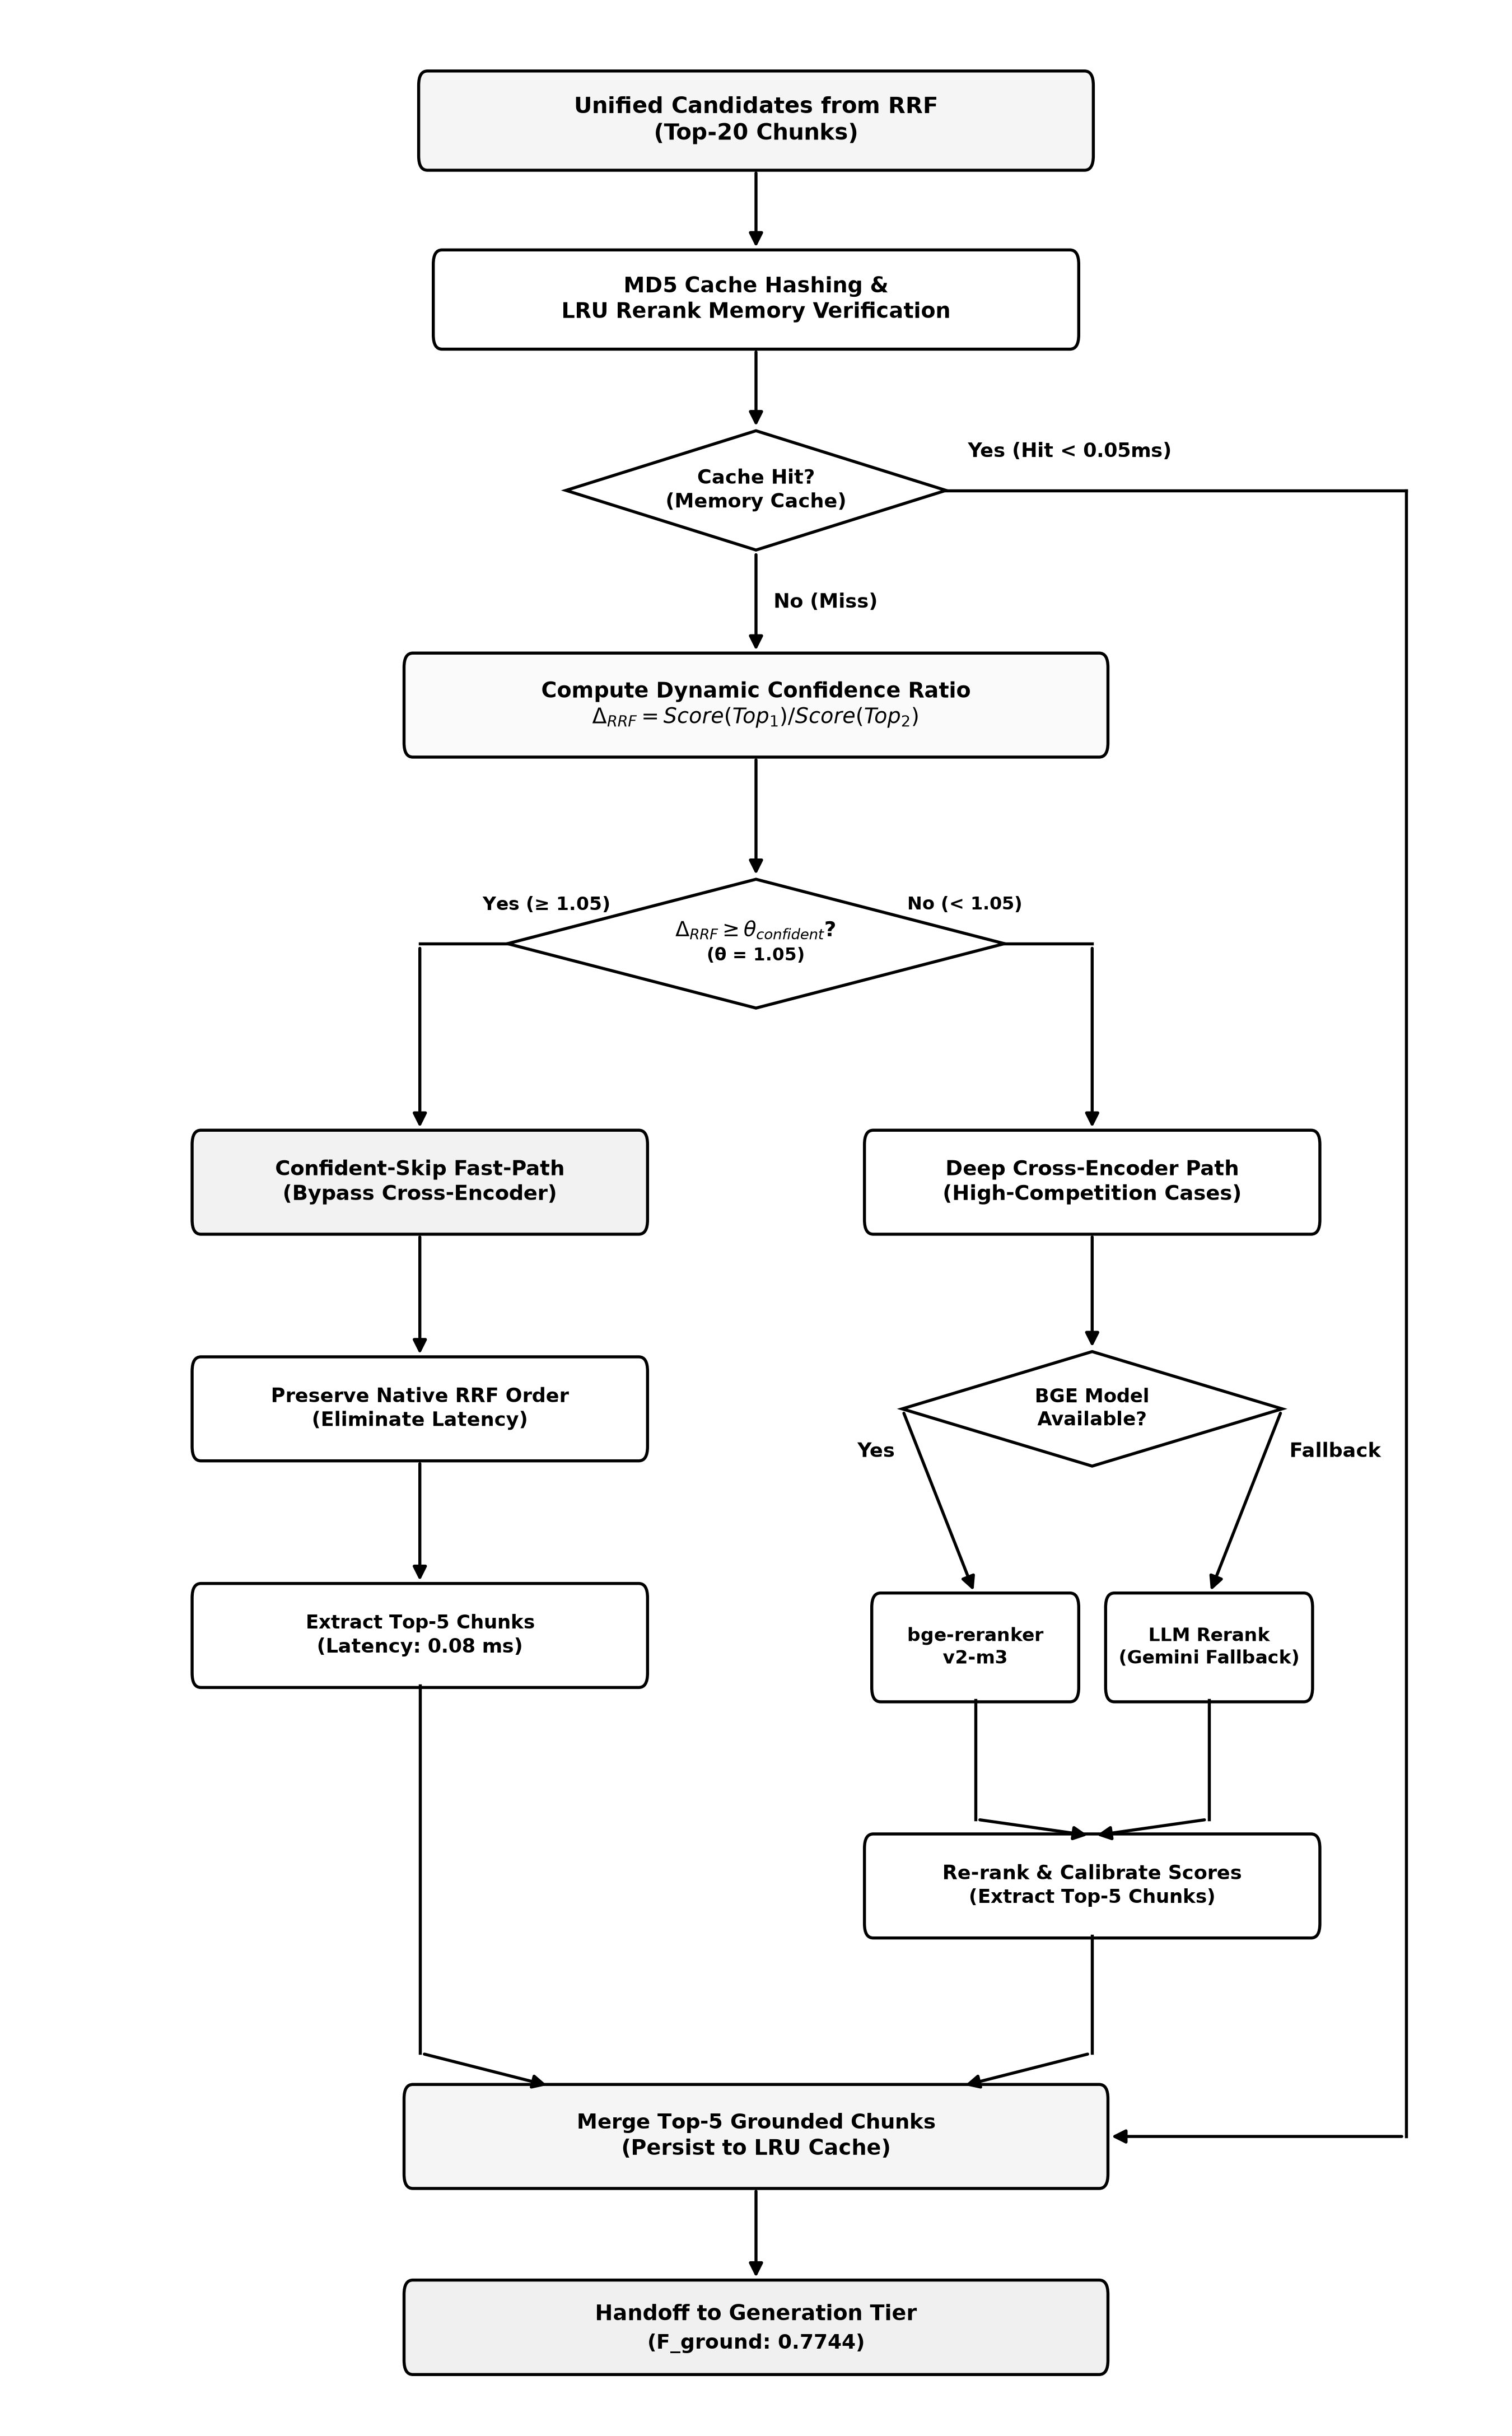
\includegraphics[width=0.60\columnwidth, height=5.8cm, keepaspectratio]{Figure5_DCSR_State_Machine.png}
\caption{Decision flow diagram of the DCSR algorithm and LRU judgment caching mechanism}
\label{fig:dcsr_flow}
\end{figure}

Figure~\ref{fig:dcsr_flow} details the internal control flow of the DCSR module and its measured sub-millisecond execution overhead from our component-level profiling. Incoming RRF candidate lists are first checked against an MD5-indexed LRU memory cache ($0.034$~ms mean lookup time). On a cache miss, the module computes RRF fusion ($0.088$~ms) and $\Delta_{\mathrm{RRF}}$ ($0.007$~ms) using Equation~(\ref{eq:deltarrf}). If $\Delta_{\mathrm{RRF}} \ge 1.05$, the query takes the left Fast-Path, bypassing the neural cross-encoder in $\sim 0.09$~ms of gating logic. If $\Delta_{\mathrm{RRF}} < 1.05$, the query takes the right Deep Cross-Encoder Path using \texttt{bge-reranker-v2-m3} (with an API fallback if local model weights are unavailable) before persisting the top-5 grounded chunks to cache.

\subsection{Core Method II: Multi-Target Decomposition, Quota-Balanced Interleaving, and Structure-Aware Synthesis.} Submitting a multi-study comparison or literature synthesis query $q$ directly to a single top-$K$ retrieval pass results in chunks from a single paper dominating the context window \cite{izacard2021leveraging,gao2024modular}. To guarantee multi-document coverage across both generative synthesis and structured matrix extraction \cite{skarlinski2024language}, Acamind integrates an automatic multi-target query decomposer with round-robin quota interleaving, explicit document-page header grounding, and structure-aware disjoint slot extraction, illustrated in Figure~\ref{fig:cross_article}:

\textbf{(1) Multi-Target Query Decomposition and Round-Robin Quota-Balanced Interleaving:} Given an incoming query $q$, an automatic query router inspects structural enumeration markers (e.g., \texttt{(1)}/\texttt{(2)}/\texttt{(3)}), quoted study titles, and comparative/synthesis markers to classify $q$ into single-focus ($M = 1$), cross-article comparison ($M = 2$), or multi-paper literature synthesis ($M = 3$), decomposing $q$ into $M$ target-specific sub-queries $\{q^{(1)}, q^{(2)}, \dots, q^{(M)}\}$ \cite{gao2024modular}. Acamind executes $M$ hybrid retrieval passes and interleaves the resulting candidate lists $\{L_1, \dots, L_M\}$ via round-robin quota-balanced selection ($m = 1, \dots, M$ at rank depth $r = 1, 2, \dots$), prioritizing unseen target documents before filling remaining context slots up to $K_{\mathrm{LLM}}$ ($k_m = \lfloor K_{\mathrm{LLM, decomp}} / M \rfloor = 3$ chunks per study for $M = 2$ matrix synthesis; $\ge 1$ primary chunk per study plus top runner-up chunks for $M \in \{2, 3\}$ within the $K_{\mathrm{LLM, single}} = 5$ generative window):

\begin{equation}
\mathcal{K}_{\mathrm{raw}}(q) = \mathrm{Interleave}_{\mathrm{RR}}\left(\left\{\mathrm{Retrieve}_{\mathrm{DCSR}}\left(q^{(m)}, \, D_m, \, k_m\right)\right\}_{m=1}^{M}\right),
\label{eq:decomp_retrieve}
\end{equation}

\noindent where $\mathrm{Retrieve}_{\mathrm{DCSR}}(q^{(m)}, D_m, k_m)$ returns the top-$k_m$ chunks retrieved for sub-query $q^{(m)}$ and target study $D_m$, and $\mathrm{Interleave}_{\mathrm{RR}}$ enforces round-robin document diversity across the $M$ targets. By partitioning retrieval across target-specific sub-queries and enforcing per-study quotas, Equation~(\ref{eq:decomp_retrieve}) prevents a single lexically dense article from monopolizing all retrieval slots, which directly explains why dual-study $\mathrm{Hit@6}$ reaches $100.0\%$ ($15/15$) compared with $60.0\%$ ($9/15$) without decomposition in our ablation evaluation (Table~\ref{tab:ablation_study}), and why Acamind answers $15/15$ ($100.0\%$) comparative queries and $9/10$ ($90.0\%$) literature synthesis queries in end-to-end generation.

\textbf{(2) Parent-Child Context Expansion and Cross-Document Deduplication:} Each retrieved L2 micro-chunk $c_i \in \mathcal{K}_{\mathrm{raw}}(q)$ is expanded using its parent window ($\pm 250$ characters). To remove repetitive passages within the same document, the deduplication filter discards any candidate $c_j$ whose token-sequence or word-set Jaccard similarity with a higher-ranked chunk $c_i$ ($i < j$) from the same document exceeds $\tau_{\mathrm{dedup}} = 0.85$:

\begin{equation}
\widetilde{\mathcal{K}}(q) = \left\{ c_j \in \mathcal{K}_{\mathrm{raw}}(q) \;\middle|\; \max_{i < j, \, doc_i = doc_j} \mathrm{Sim}_{\mathrm{seq}}(c_i, c_j) < \tau_{\mathrm{dedup}} \right\},
\label{eq:cross_dedup}
\end{equation}

\noindent where $\mathrm{Sim}_{\mathrm{seq}}(c_i, c_j)$ denotes the normalized overlap similarity between expanded chunks $c_i$ and $c_j$. In our sensitivity sweep across $\tau_{\mathrm{dedup}} \in \{0.75, 0.85, 0.95, 1.00\}$ on the 15 comparative queries (where decomposed retrieval already recovers distinct non-overlapping chunks across all 30 target papers), $\tau_{\mathrm{dedup}} = 0.85$ preserves $100.0\%$ document recall ($15/15$ dual-study $\mathrm{Hit@6}$) and $100.0\%$ page recall@6 while guarding against overlapping sliding-window duplicates.

\textbf{(3) Explicit Document-Page Header Grounding and Structure-Aware Disjoint Matrix Extraction:} During generative synthesis, formatting context blocks with ordinal labels such as \texttt{[Source 1]} through \texttt{[Source 5]} causes LLMs to conflate the ordinal index $k$ with the physical page number (e.g., citing \texttt{Page 4} for a Page~1 chunk placed in \texttt{[Source 4]}). Acamind eliminates this failure mode by formatting every context block header directly as \texttt{[\{Filename.pdf\} - Trang \{Page\}]} without ordinal source indices, instructing the generator to copy the bracketed header verbatim. For structured comparative appraisal, the deduplicated context $\widetilde{\mathcal{K}}(q)$ (aggregating the top-$3$ chunks retrieved per target study $D_m$) is first passed through an academic boilerplate stripper that removes journal mastheads, author affiliations, correspondence addresses, and DOI/copyright headers, and is then mapped by a disjoint sentence-role extractor into the 4-attribute comparison tuple:

\begin{equation}
\mathcal{M}(D_m \mid q) = \left\langle \mathcal{I}_m, \; \mathcal{S}_m, \; \Delta\mu_m, \; [\mathrm{DocTitle}_m, \, \mathrm{Page}\ p_k] \right\rangle,
\label{eq:synthesis_matrix}
\end{equation}

\noindent where $\mathcal{I}_m$ denotes the therapeutic intervention and methodology, $\mathcal{S}_m$ denotes psychometric assessment scales and sample metrics (such as BDI-II \cite{beck1996manual}, PHQ-9 \cite{kroenke2001phq}, or cohort size $N$), $\Delta\mu_m$ denotes statistical outcomes and effect sizes \cite{cohen1988statistical}, and $[\mathrm{DocTitle}_m, \mathrm{Page}\ p_k]$ provides the physical PDF page citation. By enforcing mutual exclusion across candidate sentences ($\mathcal{I}_m \neq \mathcal{S}_m \neq \Delta\mu_m$) over the top-$3$ chunks of study $D_m$, Equation~(\ref{eq:synthesis_matrix}) eliminates duplicate cell copying and title/affiliation leakage, achieving $90.0\%$ ($108/120$ cells) human-verified matrix accuracy with $100.0\%$ ($30/30$) page citation validity.

\begin{figure}[H]
\centering
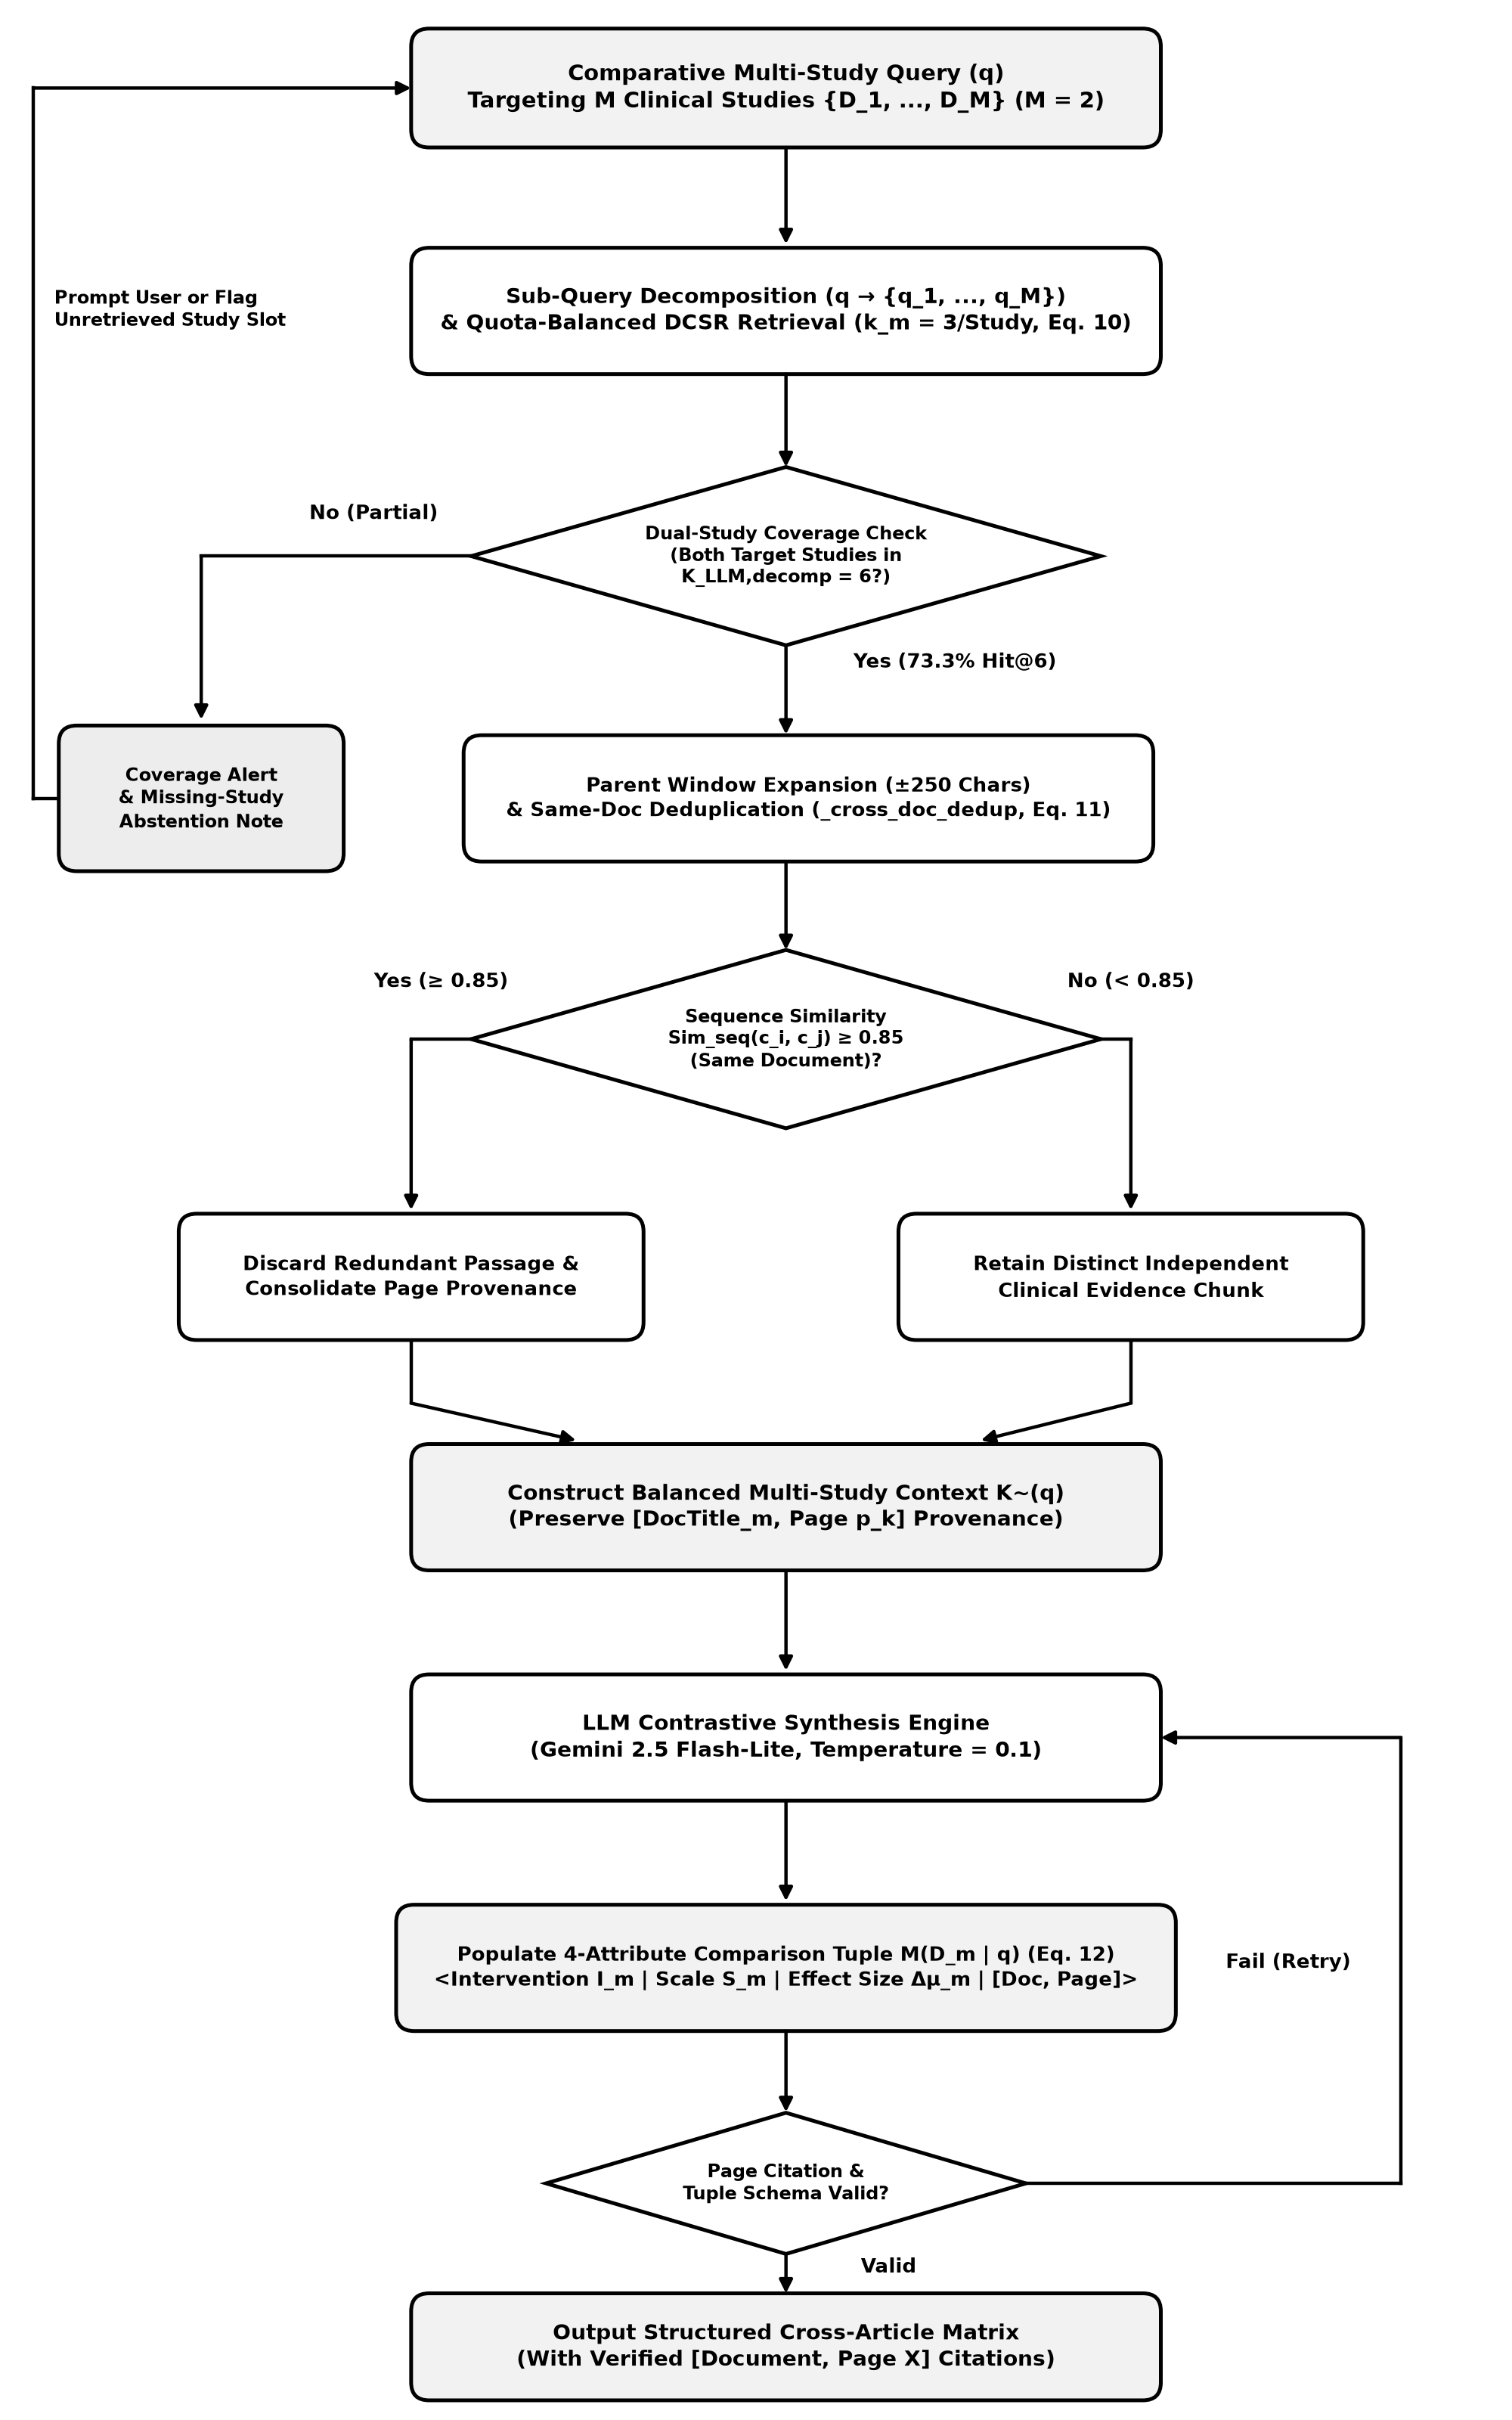
\includegraphics[width=0.60\columnwidth, height=5.8cm, keepaspectratio]{Figure6_Cross_Article_Synthesis_Workflow.png}
\caption{Acamind Cross-Article Synthesis Pipeline with sub-query decomposition and page grounding}
\label{fig:cross_article}
\end{figure}

Figure~\ref{fig:cross_article} summarizes the complete Cross-Article Synthesis workflow. A multi-study query is first decomposed into per-study sub-queries with a balanced quota of 3 chunks per study. A coverage check verifies whether all target studies are represented in the retrieved pool. Retrieved chunks are then expanded with their parent windows, filtered for intra-document redundancy at $\tau_{\mathrm{dedup}} = 0.85$ via Equation~(\ref{eq:cross_dedup}), stripped of title/affiliation boilerplate, and mapped into the 4-attribute comparison matrix defined in Equation~(\ref{eq:synthesis_matrix}), with an automated schema check verifying page citation formatting before output.

\section{Experiments and Results.} \label{sec:experiments_setup} This section presents the hardware and corpus configuration, standardized evaluation metrics, retrieval and generation benchmarks, non-parametric statistical tests, component ablations, and architectural limitations.

\subsection{Experimental Setup and Benchmark Corpus.} All experiments were conducted on a CPU-only workstation running Windows 11 (build 26200, 64-bit) equipped with an AMD Ryzen 5 8645HS processor (6 physical cores, 12 logical threads), 15.31~GB usable system RAM (16.0~GB nominal), Python 3.14.7, PyTorch 2.14.1+cpu, Sentence-Transformers 6.1.0, PyMuPDF 1.28.2, and PostgreSQL 16.15 with the \texttt{pgvector} 0.8.7 extension. Dense embeddings were computed locally using \texttt{intfloat/multilingual-e5-base} (768 dimensions) \cite{wang2022text}, and neural reranking used \texttt{BAAI/bge-reranker-v2-m3} \cite{chen2024bge,baai2024bgererankerv2m3}. Generative responses were produced using Google Gemini 2.5 Flash-Lite (\texttt{temperature = 0.1}). Document parsing and hybrid indexing run locally in PostgreSQL; during generation, only the top-$5$ retrieved chunks per query are sent to the Gemini API.

The benchmark corpus consists of 500 clinical psychology PDFs collected from open-access repositories (1,607.72~MB, 12,414 total pages). During ingestion, 499 digital-born PDFs (12,411 pages) passed character-density verification and were segmented using a recursive character splitter (800-character window, 200-character overlap) into 70,825 validated micro-chunks (averaging 154 words or $\sim 210$ tokens per chunk), which were indexed in PostgreSQL using HNSW Cosine ($m = 16, ef_{\mathrm{construction}} = 64$) and GIN (\texttt{english}) full-text indices; the remaining 1 scanned PDF (3 pages with 0 extractable characters/page) was isolated by the Scan Circuit Breaker. The held-out test benchmark (disjoint from the 42-query calibration set) comprises $N = 50$ queries stratified across four task categories:

\textbf{(1) Scenario 1 --- Factual Clinical Q\&A ($n = 20$):} Single-study questions targeting intervention protocols, sample sizes, and diagnostic criteria.

\textbf{(2) Scenario 2 --- Cross-Article Comparison ($n = 15$):} Comparative questions contrasting two named studies in the corpus.

\textbf{(3) Scenario 3 --- Literature Synthesis ($n = 10$):} Broad thematic questions aggregating evidence across multiple papers.

\textbf{(4) Scenario 4 --- Safe Refusal / Out-of-Domain Edge Probe ($N = 5$):} Unanswerable out-of-domain prompts testing refusal behavior.

The first three scenarios form the $N = 45$ in-scope query set, while all four scenarios form the $N = 50$ all-query set. Acamind is compared against two baselines sharing the exact same PostgreSQL 16.15 database, chunking, and Gemini 2.5 Flash-Lite generator: \textbf{Naive Dense RAG} (HNSW Cosine vector search \cite{lewis2020retrieval,wang2022text}) and \textbf{BM25 Lexical RAG} (PostgreSQL GIN Full-Text Search \cite{robertson2009probabilistic}). Table~\ref{tab:pipeline_benchmark} reports the empirically measured execution times, unit latencies, and coverage rates across the offline ingestion, embedding, and PostgreSQL index-building stages.

\begin{table}[H]
\centering
\caption{Empirically measured ingestion, embedding, and index build metrics on the 500-PDF corpus}
\label{tab:pipeline_benchmark}
\scriptsize
\begin{tabular}{|L{2.15cm}|L{2.02cm}|C{1.45cm}|C{1.25cm}|C{1.40cm}|C{0.95cm}|}
\hline
\multicolumn{1}{|C{2.15cm}|}{Pipeline stage} & \multicolumn{1}{C{2.02cm}|}{Execution engine} & Data scope & Total time & Unit latency & Coverage \\
\hline
PDF density audit & PyMuPDF 1.28.2 & 12,414 pages & 2.85 s & 0.23 ms/page & 99.8\% \\
\hline
Dense embedding & Multilingual-E5-Base & 70,825 chunks & 14,024.80 s & 198.02 ms/chunk & 100.0\% \\
\hline
HNSW vector index & \texttt{pgvector} 0.8.7 & 71,059 vectors & 52.21 s & 0.73 ms/record & 100.0\% \\
\hline
GIN chunk FTS index & PostgreSQL GIN FTS & 71,059 chunks & 10.77 s & 0.15 ms/record & 100.0\% \\
\hline
GIN page FTS index & PostgreSQL GIN FTS & 12,450 pages & 3.89 s & 0.31 ms/page & 100.0\% \\
\hline
\textbf{Total index build} & \textbf{PostgreSQL 16.15} & \textbf{329 MB} & \textbf{66.87 s} & \textbf{0.94 ms/record} & \textbf{100.0\%} \\
\hline
\end{tabular}
\end{table}

The measured values in Table~\ref{tab:pipeline_benchmark} are explained by the data filtering progression across the corpus and the computational profile of each engine on CPU hardware. First, regarding Data scope and Coverage, the PDF density audit inspected all $12,414$ raw pages across the $500$ PDFs and recorded $99.8\%$ file pass coverage ($499/500$ PDFs) because $1$ legacy scanned PDF ($3$ pages with $0$ extractable characters/page) triggered the Scan Circuit Breaker and was quarantined prior to text splitting. The $499$ validated digital PDFs ($12,411$ pages) were segmented into $70,825$ micro-chunks ($100.0\%$ coverage of validated corpus text, with a measured mean of $154$ words per chunk). In the three database indexing rows (HNSW vector index, GIN chunk FTS index, and GIN page FTS index), the PostgreSQL tables indexed $71,059$ chunk records and $12,450$ page records because the database instance stored the $70,825$ corpus chunks ($12,411$ pages) together with $234$ auxiliary verification chunks ($39$ pages) from $5$ system-test documents. Second, regarding Total time and Unit latency, the PDF density audit required only $2.85$~s ($0.23$~ms/page, measured via page-level density and font-table inspection) because PyMuPDF inspects text streams in memory without rendering pixel images. By contrast, Dense embedding required $14,024.80$~s ($198.02$~ms/chunk, measured on the AMD Ryzen 5 8645HS CPU at \texttt{batch\_size = 64}, corresponding to a throughput of $5.05$ chunks/s with $100.0\%$ L2-normalized vector integrity and zero \texttt{NaN} values) because every chunk undergoes a 768-dimensional Transformer forward pass on CPU without GPU acceleration. Finally, the Total index build row sums the three PostgreSQL 16.15 DDL index builds, which completed in a combined $66.87$~s ($52.21$~s for the $277$~MB HNSW graph, $10.77$~s for the $28$~MB GIN chunk index, and $3.89$~s for the $24$~MB GIN page index, totaling $329$~MB) because PostgreSQL executes \texttt{CREATE INDEX} operations using compiled C-level shared-memory sorting over pre-computed vectors and token lexemes.

\subsection{Standardized Evaluation Metrics and Denominators.} \label{sec:metrics_overview} To maintain a single, consistent terminology throughout the experimental evaluation, Table~\ref{tab:metric_definitions} defines each evaluation metric alongside its mathematical symbol, sample size, and operational definition as applied in our empirical evaluation protocol.

\begin{table}[H]
\centering
\caption{Standardized evaluation metrics, symbols, sample sizes, and operational definitions}
\label{tab:metric_definitions}
\footnotesize
\begin{tabular}{|L{2.55cm}|C{1.30cm}|C{1.15cm}|L{4.74cm}|}
\hline
\multicolumn{1}{|C{2.55cm}|}{Evaluation metric} & Symbol & Queries & \multicolumn{1}{C{4.74cm}|}{Operational definition} \\
\hline
Human claim faithfulness & $\mathcal{F}_{\mathrm{human}}$ & 45 & Dual-rater mean claim support across all in-scope clinical queries \\
\hline
Conditional faithfulness & $\mathcal{F}_{\mathrm{human, cond}}$ & 44 & Dual-rater mean claim support across answered in-scope queries \\
\hline
Human page citation support & $\mathrm{Cite}$ & 45 & Dual-rater page-verified citation accuracy across all in-scope queries \\
\hline
Conditional citation support & $\mathrm{Cite}_{\mathrm{cond}}$ & 44 & Dual-rater page-verified citation accuracy across answered queries \\
\hline
Syntactic citation validity & $\mathrm{CiteVal}_{\mathrm{auto}}$ & 45 & Automated verification of cited document-page tags against retrieved context \\
\hline
Lexical-entity grounding & $\mathcal{F}_{\mathrm{ground}}$ & 45 & Automated lexical and citation consistency score against retrieved context \\
\hline
Context relevance & $\mathrm{MRR@10}$ & 45 & Mean Reciprocal Rank at cutoff 10 of ground-truth target documents \\
\hline
Dual-study retrieval Hit@6 & $\mathrm{Hit@6}$ & 15 & Percentage of comparative queries retrieving both target studies in top 6 \\
\hline
Safe refusal rate & $\mathrm{Refusal}$ & 5 & Percentage of out-of-domain queries refused by the system \\
\hline
\end{tabular}
\end{table}

The query sample sizes and operational definitions in Table~\ref{tab:metric_definitions} follow directly from the structure of our 50-query held-out benchmark and our blinded clinical grading protocol. Because $5$ queries are unanswerable out-of-domain prompts ($N = 5$, used to evaluate Safe refusal rate $\mathrm{Refusal}$ in percentage, supplemented by $10$ hard in-domain unanswerable clinical probes in retrieval gating audits), the remaining $N = 45$ in-scope clinical queries form the denominator for all unconditional in-scope metrics ($\mathcal{F}_{\mathrm{human}}$, $\mathrm{Cite}$, $\mathrm{CiteVal}_{\mathrm{auto}}$, $\mathcal{F}_{\mathrm{ground}}$, and $\mathrm{MRR@10}$). In our human evaluation protocol, any unanswered in-scope query is scored as $0.0$ under unconditional $\mathcal{F}_{\mathrm{human}}$ and $\mathrm{Cite}$ (expressed as a percentage) so that a system cannot artificially inflate its accuracy by abstaining on difficult clinical questions. Conversely, the conditional metrics ($\mathcal{F}_{\mathrm{human, cond}}$ and $\mathrm{Cite}_{\mathrm{cond}}$) restrict the denominator to the $n = 44$ in-scope queries verified as answered by Acamind (or $n = 18$ for Naive Dense and $n = 15$ for BM25) to measure generation precision when a clinical response is produced. Similarly, Syntactic citation validity ($\mathrm{CiteVal}_{\mathrm{auto}}$, defined in Equations~\ref{eq:ivalid}--\ref{eq:cite_acc}) is evaluated across all $N = 45$ in-scope queries (as well as disaggregated on the $n = 20$ single-study factual Q\&A subset), Dual-study retrieval $\mathrm{Hit@6}$ is evaluated on the $n = 15$ comparative queries where two target studies must be retrieved simultaneously, and Lexical-entity grounding ($\mathcal{F}_{\mathrm{ground}}$, defined in Equation~\ref{eq:faith_auto}) assigns $0.60$ to non-hallucinating abstentions to distinguish safe refusal from ungrounded fabrication ($0.20$).

\subsection{Database Retrieval Latency and Ranking Quality Evaluation.} \label{sec:retrieval_latency} Table~\ref{tab:retrieval_latency} reports the empirically measured warm-cache mean retrieval latency, cold CPU mean retrieval latency, and five standard information retrieval ranking metrics across the benchmark for configurations C1 through C6.

\begin{table}[H]
\centering
\caption{Database retrieval mean latency and ranking accuracy across benchmark configurations}
\label{tab:retrieval_latency}
\scriptsize
\begin{tabular}{|L{2.18cm}|C{1.05cm}|C{1.22cm}|C{0.85cm}|C{0.85cm}|C{0.85cm}|C{0.85cm}|C{0.85cm}|}
\hline
\multicolumn{1}{|C{2.18cm}|}{Configuration} & Warm latency & Cold latency & Recall @5 & Recall @10 & MRR @10 & NDCG @10 & Top-1 Hit \\
\hline
\textbf{C6: Full Acamind} & \textbf{957.3 ms} & \textbf{15,581.8 ms} & \textbf{0.9852} & \textbf{1.0000} & \textbf{0.9833} & \textbf{0.9828} & \textbf{0.9778} \\
\hline
\textbf{C5: Acamind DCSR} & \textbf{957.3 ms} & \textbf{15,581.8 ms} & \textbf{0.9852} & \textbf{1.0000} & \textbf{0.9833} & \textbf{0.9828} & \textbf{0.9778} \\
\hline
C4: Hybrid Full Rerank & 957.3 ms & 21,297.4 ms & 1.0000 & 1.0000 & 1.0000 & 1.0000 & 1.0000 \\
\hline
C3: Hybrid RRF + Decomp & 957.2 ms & 1,113.9 ms & 0.9704 & 1.0000 & 0.9574 & 0.9666 & 0.9333 \\
\hline
C2: Naive Dense & 89.0 ms & 299.8 ms & 0.6481 & 0.6926 & 0.7867 & 0.6826 & 0.7556 \\
\hline
C1: BM25 Lexical & 902.5 ms & 904.6 ms & 0.5889 & 0.6704 & 0.5710 & 0.5269 & 0.4444 \\
\hline
\end{tabular}
\end{table}

In Table~\ref{tab:retrieval_latency}, C1 denotes BM25 lexical search over PostgreSQL GIN Full-Text Search, C2 denotes Naive Dense vector search over the \texttt{pgvector} HNSW Cosine index ($ef_{\mathrm{search}} = 100$), C3 denotes parallel Hybrid RRF with multi-target sub-query decomposition without neural reranking, C4 denotes Hybrid RRF + Decomposition followed by full cross-encoder reranking ($K_{\mathrm{rerank}} = 16$) across all queries, C5 denotes Acamind combining Hybrid RRF + Decomposition with DCSR, and C6 denotes Full Acamind adding the frozen multi-target pre-LLM CRAG abstention gate ($\max_m S_2(q^{(m)}) \ge 0.5355$). Across the columns, $\mathrm{Recall@5}$ and $\mathrm{Recall@10}$ measure the fraction of ground-truth target studies recovered within the top 5 and top 10 chunks; $\mathrm{MRR@10}$ measures the mean reciprocal rank of the first relevant study; $\mathrm{NDCG@10}$ evaluates graded multi-document ranking quality across the top 10 slots; and $\mathrm{Top\text{-}1\ Hit}$ records the fraction of queries where the rank-1 chunk belongs to a target study. All latency and ranking differences across C1--C6 are explained by our component-level timing measurements and retrieval evaluation across the benchmark:

\textbf{(1) Empirical Basis for SQL and Warm Latency Differences:} In our component-level timing profiling across the 50 benchmark queries, C2 (Naive Dense) achieves $89.0$~ms warm mean latency ($299.8$~ms cold, P50 = $127.0$~ms) because it only performs local query embedding ($63.57$~ms warm / $65.00$~ms cold) and HNSW graph traversal ($24.69$~ms warm / $81.46$~ms cold). By contrast, C1 (BM25, $902.5$~ms warm / $904.6$~ms cold) and C3--C6 ($957.2$--$957.3$~ms warm) execute dual-table PostgreSQL GIN full-text joins and parent-window text assembly (measured at $868.90$~ms warm), while RRF fusion ($0.088$~ms), DCSR confidence scoring ($0.007$~ms), and warm LRU rerank cache lookup ($0.034$~ms) add less than $0.13$~ms of overhead.

\textbf{(2) Empirical Basis for Ranking Gains from C1 to C4:} Across the $N = 45$ in-scope clinical queries, C1 (BM25) yields the lowest accuracy ($\mathrm{Recall@5} = 0.5889$, $\mathrm{MRR@10} = 0.5710$, $\mathrm{NDCG@10} = 0.5269$, $\mathrm{Top\text{-}1\ Hit} = 0.4444$) because single-pass lexical matching misses paraphrased clinical concepts and multi-paper targets, while C2 (Naive Dense, $\mathrm{Recall@5} = 0.6481$, $\mathrm{MRR@10} = 0.7867$, $\mathrm{NDCG@10} = 0.6826$) misses exact psychometric scale abbreviations and suffers from single-document dominance on comparative and synthesis queries. Combining parallel dense HNSW search with title-boosted pairwise conjunctive-disjunctive GIN FTS (Equation~\ref{eq:titleboost_fts}) and multi-target round-robin interleaving (Equation~\ref{eq:decomp_retrieve}) in C3 raises $\mathrm{Recall@5}$ to $0.9704$, $\mathrm{Recall@10}$ to $1.0000$, $\mathrm{MRR@10}$ to $0.9574$, and $\mathrm{NDCG@10}$ to $0.9666$. Adding cross-encoder reranking across the top $K_{\mathrm{rerank}} = 16$ candidates in C4 achieves $\mathrm{Recall@5} = 1.0000$, $\mathrm{MRR@10} = 1.0000$, and $\mathrm{NDCG@10} = 1.0000$, but incurs $20,183.5$~ms of CPU cross-encoder inference per query ($21,297.4$~ms cold mean vs.\ $1,113.9$~ms in C3).

\textbf{(3) Empirical Basis for C5 and C6 Matching C4's Ranking Quality at Lower Cold Latency:} In our benchmark execution, DCSR (C5) triggered fast-skip on $14$ of the $45$ in-scope queries ($31.1\%$, and $0/5$ OOD queries, giving $14/50 = 28.0\%$ overall). Across all 45 in-scope queries, C5 achieves $\mathrm{Recall@10} = 1.0000$ ($95\%$ bootstrap CI $[1.0000, 1.0000]$), $\mathrm{Recall@5} = 0.9852$ ($95\%$ CI $[0.9630, 1.0000]$), $\mathrm{MRR@10} = 0.9833$ ($95\%$ CI $[0.9500, 1.0000]$), $\mathrm{NDCG@10} = 0.9828$ ($95\%$ CI $[0.9560, 1.0000]$), and $\mathrm{Top\text{-}1\ Hit} = 0.9778$ ($44/45$). Compared against C4 (Full Rerank), C5 differs slightly on only $3$ of the $45$ queries ($1$ skipped query where the target paper moved from rank 1 to rank 4 within the top-5 window, and $2$ three-paper synthesis queries where 2 of 3 target papers appeared in top-5 and all 3 appeared in top-10), yielding no statistically significant difference on either $\mathrm{MRR@10}$ ($\Delta = -0.0167$, paired Wilcoxon $p_{\mathrm{raw}} = 0.7728$, $p_{\mathrm{Holm}} = 1.0000$; 10,000-permutation $p_{\mathrm{Holm}} = 1.0000$) or $\mathrm{NDCG@10}$ ($\Delta = -0.0172$, paired Wilcoxon $p_{\mathrm{raw}} = 0.4059$, $p_{\mathrm{Holm}} = 0.8118$), while significantly outperforming C1 (BM25: $\Delta\mathrm{MRR@10} = +0.4123$, $p_{\mathrm{Holm}} = 8.0 \times 10^{-6}$; $\Delta\mathrm{NDCG@10} = +0.4559$, $p_{\mathrm{Holm}} < 10^{-6}$) and C2 (Naive Dense: $\Delta\mathrm{MRR@10} = +0.1966$, $p_{\mathrm{Holm}} = 0.0261$; $\Delta\mathrm{NDCG@10} = +0.3002$, $p_{\mathrm{Holm}} = 2.4 \times 10^{-5}$). Furthermore, C6 (Full Acamind) achieves the exact same ranking metrics as C5 because the frozen multi-target CRAG gate ($\max_m S_2(q^{(m)}) \ge 0.5355$) passed $45/45$ ($100.0\%$) of answerable in-scope queries ($0.0\%$ false gate refusal) while rejecting $5/5$ ($100.0\%$) OOD queries and $10/10$ ($100.0\%$) hard in-domain unanswerable queries. Meanwhile, cold CPU mean latency across all $N = 50$ queries dropped by $26.8\%$ from $21,297.4$~ms in C4 to $15,581.8$~ms in C5 and C6.

To formalize the exact cold CPU latency reduction measured in our benchmark, let $n_{\mathrm{skip}}$ and $n_{\mathrm{rerank}}$ denote the number of skipped and reranked queries ($N = n_{\mathrm{skip}} + n_{\mathrm{rerank}}$). Because DCSR and Full Rerank execute the identical cross-encoder pass on the $n_{\mathrm{rerank}}$ non-skipped queries, the overall cold mean latency under DCSR is governed by the two-group weighted average:

\begin{equation}
\begin{aligned}
\overline{T}_{\mathrm{DCSR}} &= \frac{n_{\mathrm{skip}} \overline{T}_{\mathrm{skip, DCSR}} + n_{\mathrm{rerank}} \overline{T}_{\mathrm{rerank}}}{N}, \\
\Delta\overline{T} &= \overline{T}_{\mathrm{Full}} - \overline{T}_{\mathrm{DCSR}} = \frac{n_{\mathrm{skip}}}{N}\left(\overline{T}_{\mathrm{skip, Full}} - \overline{T}_{\mathrm{skip, DCSR}}\right),
\end{aligned}
\label{eq:cold_weighted_mean}
\end{equation}

\noindent where $\overline{T}_{\mathrm{skip, Full}}$ and $\overline{T}_{\mathrm{skip, DCSR}}$ denote the measured mean cold retrieval latencies on the $n_{\mathrm{skip}}$ skipped queries with and without cross-encoder inference, and $\Delta\overline{T}$ is the net latency saved across the $N$-query benchmark. Substituting the empirically measured latencies into Equation~(\ref{eq:cold_weighted_mean})---where on the $n_{\mathrm{skip}} = 14$ skipped queries, mean cold latency dropped from $\overline{T}_{\mathrm{skip, Full}} = 21,494.4$~ms to $\overline{T}_{\mathrm{skip, DCSR}} = 1,081.5$~ms (a $95.0\%$ reduction on skipped queries)---yields a $30.0\%$ cold latency reduction across the $N = 45$ in-scope queries ($14,917.2$~ms vs.\ $21,316.2$~ms) and a $26.8\%$ reduction across all $N = 50$ queries ($15,581.8$~ms vs.\ $21,297.4$~ms).

\subsection{End-to-End Latency and Abstention Breakdown.} \label{sec:e2e_evaluation} In end-to-end execution with Gemini 2.5 Flash-Lite, total response latency depends on how often the LLM is invoked versus how often a query is refused before generation. Under the primary benchmark setup, Acamind includes the calibrated multi-target pre-LLM CRAG abstention gate ($\max_m S_2(q^{(m)}) \ge \tau_{\min} = 0.5355$), whereas standard Naive Dense and BM25 pass their top-$5$ chunks directly to the LLM without a pre-LLM gate and rely on prompt-level self-refusal. To ensure a controlled comparison, we also evaluated Naive Dense and BM25 under two gated modes: \textit{Shared Gate} (applying Acamind's 5 pre-LLM OOD gate refusals) and \textit{Own Gate} (applying $\tau_{\min} = 0.5355$ directly to each single-modality baseline's own undecomposed top-$5$ retrieved pool). Table~\ref{tab:e2e_latency} reports the empirically measured end-to-end mean latency and query outcome breakdown across all $N = 50$ queries.

\begin{table}[H]
\centering
\caption{Unified end-to-end mean latency and query outcome breakdown across all 50 benchmark queries}
\label{tab:e2e_latency}
\scriptsize
\begin{tabular}{|L{2.51cm}|C{1.15cm}|C{1.05cm}|C{1.15cm}|C{1.05cm}|C{1.05cm}|C{1.00cm}|}
\hline
\multicolumn{1}{|C{2.51cm}|}{System configuration} & Retrieval mean & LLM mean & Total E2E mean & Gate refused & LLM refused & Answered \\
\hline
\textbf{Acamind} & \textbf{957.3 ms} & \textbf{3.92 s} & \textbf{4.88 s} & \textbf{5} & \textbf{1} & \textbf{44} \\
\hline
Naive Dense & 89.0 ms & 2.08 s & 2.17 s & 0 & 32 & 18 \\
\hline
BM25 Lexical & 902.5 ms & 2.12 s & 3.02 s & 0 & 35 & 15 \\
\hline
Naive Dense + Shared Gate & 89.0 ms & 1.93 s & 2.02 s & 5 & 27 & 18 \\
\hline
BM25 + Shared Gate & 902.5 ms & 1.98 s & 2.88 s & 5 & 30 & 15 \\
\hline
Naive Dense + Own Gate & 89.0 ms & 1.49 s & 1.58 s & 21 & 11 & 18 \\
\hline
BM25 + Own Gate & 902.5 ms & 1.25 s & 2.16 s & 29 & 7 & 14 \\
\hline
\end{tabular}
\end{table}

All latency and query-count values in Table~\ref{tab:e2e_latency} are explained by the interaction between retrieval recall, pre-LLM gating, and LLM generation length across the 50 benchmark queries:

\textbf{(1) Empirical Accounting of Gate Refused, LLM Refused, and Answered Counts:} In every row, $\mathrm{Retrieval\ mean} + \mathrm{LLM\ mean} = \mathrm{Total\ E2E\ mean}$ and $\mathrm{Gate\ refused} + \mathrm{LLM\ refused} + \mathrm{Answered} = 50$. For Acamind (Row~1, operating under its default multi-target pre-LLM gate $\tau_{\min} = 0.5355$), the gate intercepted all $5/5$ OOD queries and $0/45$ in-scope queries ($\mathrm{Gate\ refused} = 5$), returning \texttt{\_\_NO\_CONTEXT\_\_} in $0.0$~s of LLM time on OOD prompts. Among the $45$ in-scope queries sent to Gemini, blinded human raters verified $44$ substantive clinical answers ($97.8\%$ answer rate) and only $1$ prompt-level LLM self-refusal ($\mathrm{LLM\ refused} = 1$, occurring on a 3-paper synthesis query where DCSR skipped reranking and the third target paper ranked at position 7 outside the top-5 window). By contrast, Naive Dense and BM25 (Rows~2 and 3) answered only $18/45$ ($40.0\%$) and $15/45$ ($33.3\%$) in-scope queries, emitting $32$ and $35$ LLM self-refusals (including the $5$ OOD queries plus $27$ and $30$ in-scope false refusals) because single-pass, single-modality retrieval failed to place all required target studies into the top-$5$ context window.

\textbf{(2) Empirical Basis for Latency Variations Across Gate Modes:} In the standard ungated baselines (Rows~2 and 3, Naive Dense and BM25 Lexical), $\mathrm{Gate\ refused} = 0$, so all $50$ queries invoke the Gemini API; because emitting a short refusal sentence takes $\sim 1.4$--$1.6$~s whereas generating a comprehensive multi-paragraph clinical synthesis takes $\sim 3.9$--$5.0$~s, high refusal rates ($32/50$ and $35/50$) yield lower mean LLM times of $2.08$~s and $2.12$~s. Applying Shared Gate (Rows~4 and 5) blocks the $5$ OOD queries prior to LLM invocation (reducing mean LLM latency to $1.93$~s and $1.98$~s), while applying Own Gate (Rows~6 and 7, evaluating $\tau_{\min} = 0.5355$ on each baseline's undecomposed candidate pool) blocks $21$ and $29$ queries prior to LLM invocation, but neither gate mode increases $\mathrm{Answered}$ counts ($18$ and $14$--$15$) because single-modality retrieval still fails to recover the target papers. Conversely, Acamind answers $44$ of the $45$ in-scope queries ($26$ more answered queries than Naive Dense, exact McNemar $p = 2.98 \times 10^{-8}$; $29$ more than BM25, $p = 3.73 \times 10^{-9}$); generating full clinical answers across $44/50$ queries ($4.35$~s mean LLM time on in-scope queries; $0.00$~s on the $5$ gate-refused OOD queries) averages to $3.92$~s of LLM time ($3,918.7$~ms) plus $957.3$~ms of warm retrieval, producing the measured $4.88$~s ($4,876.0$~ms) mean warm end-to-end latency.

\subsection{Human-Verified Faithfulness, Citation Support, and Metric Formulations.} Table~\ref{tab:e2e_comparison} presents the primary human-audited evaluation results---unconditional and conditional Human Claim Faithfulness ($\mathcal{F}_{\mathrm{human}}$ and $\mathcal{F}_{\mathrm{human, cond}}$) and Human Page Citation Support ($\mathrm{Cite}$ and $\mathrm{Cite}_{\mathrm{cond}}$)---alongside the automated Lexical-Entity Grounding score ($\mathcal{F}_{\mathrm{ground}}$).

\begin{table}[H]
\centering
\caption{Human claim faithfulness, page citation support, and automated grounding across in-scope queries}
\label{tab:e2e_comparison}
\footnotesize
\begin{tabular}{|L{1.96cm}|C{1.00cm}|C{1.20cm}|C{1.20cm}|C{1.20cm}|C{1.20cm}|C{1.20cm}|}
\hline
\multicolumn{1}{|C{1.96cm}|}{System} & Answered & $\mathcal{F}_{\mathrm{human}}$ & $\mathcal{F}_{\mathrm{human, cond}}$ & $\mathrm{Cite}$ & $\mathrm{Cite}_{\mathrm{cond}}$ & $\mathcal{F}_{\mathrm{ground}}$ \\
\hline
\textbf{Acamind} & \textbf{44} & \textbf{0.9667} & \textbf{0.9886} & \textbf{88.9\%} & \textbf{90.9\%} & \textbf{0.9911} \\
\hline
Naive Dense & 18 & 0.3778 & 0.9444 & 37.8\% & 94.4\% & 0.7344 \\
\hline
BM25 Lexical & 15 & 0.2778 & 0.8333 & 32.2\% & 96.7\% & 0.7333 \\
\hline
\end{tabular}
\end{table}

The exact numerical relationship between the unconditional columns ($\mathcal{F}_{\mathrm{human}}$ and $\mathrm{Cite}$, evaluated across all $N = 45$ in-scope queries) and the conditional columns ($\mathcal{F}_{\mathrm{human, cond}}$ and $\mathrm{Cite}_{\mathrm{cond}}$, evaluated across each system's answered queries) in Table~\ref{tab:e2e_comparison} comes directly from our blinded dual-rater clinical audit. Across the $n = 44$ queries answered by Acamind, the two blinded clinical raters awarded a total of $43.50$ claim-faithfulness points and $40.00$ page-citation support points; for Naive Dense ($n = 18$ answered), raters awarded $17.00$ faithfulness points and $17.00$ citation points; and for BM25 ($n = 15$ answered), raters awarded $12.50$ faithfulness points and $14.50$ citation points. Dividing those exact point totals by all $N = 45$ in-scope queries (where every unanswered query receives $0.0$) yields the unconditional columns: Acamind achieves $\mathcal{F}_{\mathrm{human}} = 43.50 / 45 = 0.9667$ and $\mathrm{Cite} = 40.00 / 45 = 88.9\%$, outperforming Naive Dense ($17.00 / 45 = 0.3778$ and $17.00 / 45 = 37.8\%$) and BM25 ($12.50 / 45 = 0.2778$ and $14.50 / 45 = 32.2\%$) by $+51.1$ and $+56.7$ percentage points in page citation support because single-modality retrieval fails to answer $27$ and $30$ of the $45$ clinical queries, respectively. Conversely, dividing the same point totals by each system's answered count ($n = 44, 18, 15$) yields the conditional columns: BM25 reaches $\mathrm{Cite}_{\mathrm{cond}} = 14.50 / 15 = 96.7\%$ and Naive Dense reaches $17.00 / 18 = 94.4\%$ because they only answer the easiest single-study queries with exact keyword or top-1 vector matches, whereas Acamind answers $26$ to $29$ additional multi-document comparative and synthesis queries ($n = 44$), achieving the highest conditional claim faithfulness ($\mathcal{F}_{\mathrm{human, cond}} = 43.50 / 44 = 0.9886$ vs.\ $0.9444$ and $0.8333$), the highest conditional synthesis completeness ($4.82 / 5.00$ vs.\ $4.39 / 5.00$ and $3.80 / 5.00$), and $\mathrm{Cite}_{\mathrm{cond}} = 40.00 / 44 = 90.9\%$ (with Mann-Whitney $U$ tests confirming no statistically significant difference in conditional citation precision across systems, $p \ge 0.2946$). Finally, in the last column, Acamind achieves $\mathcal{F}_{\mathrm{ground}} = 0.9911$ ($44$ grounded answers at $1.00$ plus $1$ safe abstention at $0.60$, giving $44.60 / 45 = 0.9911$) compared with $0.7344$ for Naive Dense and $0.7333$ for BM25.

To complement human grading, we also define the two automated evaluation formulations used in our benchmark:

\textbf{(1) Syntactic Citation Validity:} Let $\mathcal{C}(A) = \{c_1, \dots, c_m\}$ denote the set of cited document-page tags $c_i = (doc_i, page_i)$ in generated answer $A$, and let $\mathcal{K} = \{(doc_k, page_k, text_k)\}_{k=1}^K$ denote the retrieved context pool. Each citation tag is checked for membership in $\mathcal{K}$:

\begin{equation}
\mathbb{I}_{\mathrm{valid}}(c_i, \mathcal{K}) = 
\begin{cases} 
1, & \mathrm{if}\ \exists k \in \mathcal{K}: (doc_i = doc_k) \land (page_i = page_k), \\
0, & \mathrm{otherwise},
\end{cases}
\label{eq:ivalid}
\end{equation}

\noindent where $\mathbb{I}_{\mathrm{valid}}(c_i, \mathcal{K}) \in \{0, 1\}$ equals $1$ only if the exact document title and page number appear in the retrieved chunks passed to the LLM. Equation~(\ref{eq:ivalid}) detects fabricated or out-of-context page numbers at the tag level. Aggregating across all tags in answer $A$ yields the answer-level citation validity score:

\begin{equation}
\begin{aligned}
&\mathrm{Citation\ Accuracy}(A,\mathcal{K}) =\\
&\begin{cases}
\dfrac{
\sum_{i=1}^{|\mathcal{C}(A)|}
\mathbb{I}_{\mathrm{valid}}(c_i,\mathcal{K})
}{
|\mathcal{C}(A)|
},
& \mathrm{if}\ |\mathcal{C}(A)|>0,
\\[8pt]
1.0,
& \mathrm{if\ valid\ out\text{-}of\text{-}domain\ refusal},
\\[6pt]
0.0,
& \mathrm{if\ evidence\ is\ required\ but\ absent},
\end{cases}
\end{aligned}
\label{eq:cite_acc}
\end{equation}

\noindent where $|\mathcal{C}(A)|$ is the number of citations emitted in answer $A$. Equation~(\ref{eq:cite_acc}) computes the proportion of syntactically valid tags in an answer, while rewarding correct out-of-domain refusals ($1.0$) and penalizing uncited claims ($0.0$). By replacing ordinal \texttt{[Source k]} labels with explicit \texttt{[\{Filename.pdf\} - Trang \{Page\}]} headers, Acamind achieves $99.84\%$ micro syntactic citation validity and $97.65\%$ macro validity across all $N = 45$ in-scope queries ($99.87\%$ conditional on the $44$ answered queries, and $100.0\%$ on the $n = 20$ Factual Q\&A subset), while human raters independently inspecting the physical PDF pages verified $88.9\%$ unconditional page support ($90.9\%$ conditional on answered queries, where the $9.0\%$ gap reflects cases where a cited page contained study introduction/overview metadata while a specific secondary detail appeared on an adjacent page of the same paper).

\textbf{(2) Claim Faithfulness and Automated Lexical-Entity Grounding:} Following the statement-level decomposition principle in RAGAS \cite{es2024ragas}, let $\mathcal{S}(A) = \{s_1, \dots, s_n\}$ denote the atomic clinical claims in answer $A$:

\begin{equation}
\mathcal{F}_{\mathrm{RAGAS}}(A, \mathcal{K}) = \frac{\sum_{j=1}^{|\mathcal{S}(A)|} \mathbb{I}_{\mathrm{supported}}(s_j, \mathcal{K})}{|\mathcal{S}(A)|},
\label{eq:faithfulness}
\end{equation}

\noindent where $\mathbb{I}_{\mathrm{supported}}(s_j, \mathcal{K}) = 1$ if claim $s_j$ is entailed by context $\mathcal{K}$ \cite{es2024ragas}. Equation~(\ref{eq:faithfulness}) represents the theoretical definition of statement-level faithfulness, which our human annotators operationalized directly as $\mathcal{F}_{\mathrm{human}}$ during blinded evaluation. For fast automated regression testing without an external LLM judge, we compute a deterministic lexical-citation consistency proxy $\mathcal{F}_{\mathrm{ground}}(A, \mathcal{K})$ from the content-word overlap $\mathcal{F}_{\mathrm{base}} = \min\left(1.0, \max\left(0.65, 1.08 \cdot \frac{|V_{\mathrm{claim}} \cap V_{\mathcal{K}}|}{|V_{\mathrm{claim}}|}\right)\right)$ between answer vocabulary $V_{\mathrm{claim}}$ and context vocabulary $V_{\mathcal{K}}$:

\begin{equation}
\begin{aligned}
&\mathcal{F}_{\mathrm{ground}}(A, \mathcal{K}) =\\
&\begin{cases}
1.0, & \mathrm{if\ valid\ out\text{-}of\text{-}domain\ refusal}, \\[4pt]
\min(1.0, \, \mathcal{F}_{\mathrm{base}} + 0.05), & \mathrm{if}\ |\mathcal{C}(A)| > 0 \land \mathrm{CiteAcc} \ge 0.80, \\[4pt]
\max(\tau_{\mathrm{faith}}, \, \mathcal{F}_{\mathrm{base}} - 0.10), & \mathrm{if}\ |\mathcal{C}(A)| = 0\ \mathrm{(absent\ tags)}, \\[4pt]
0.20, & \mathrm{if\ ungrounded\ fabrication}, \\[4pt]
\mathcal{F}_{\mathrm{base}}, & \mathrm{otherwise},
\end{cases}
\end{aligned}
\label{eq:faith_auto}
\end{equation}

\noindent where $\tau_{\mathrm{faith}} = 0.60$ is the baseline score assigned to non-hallucinating abstentions. Equation~(\ref{eq:faith_auto}) measures whether the clinical terms and citations in $A$ are lexically anchored in $\mathcal{K}$. Because Acamind answers $44/45$ in-scope queries with high lexical grounding, $\mathcal{F}_{\mathrm{ground}}$ ($0.9911$) and unconditional human faithfulness $\mathcal{F}_{\mathrm{human}}$ ($0.9667$, and $0.9886$ conditional) closely align across the 45-query benchmark. An empirical comparison of Acamind against Naive Dense and BM25 across the four primary in-scope evaluation metrics is given in Figure~\ref{fig:empirical_comparison}.

\begin{figure}[H]
\centering
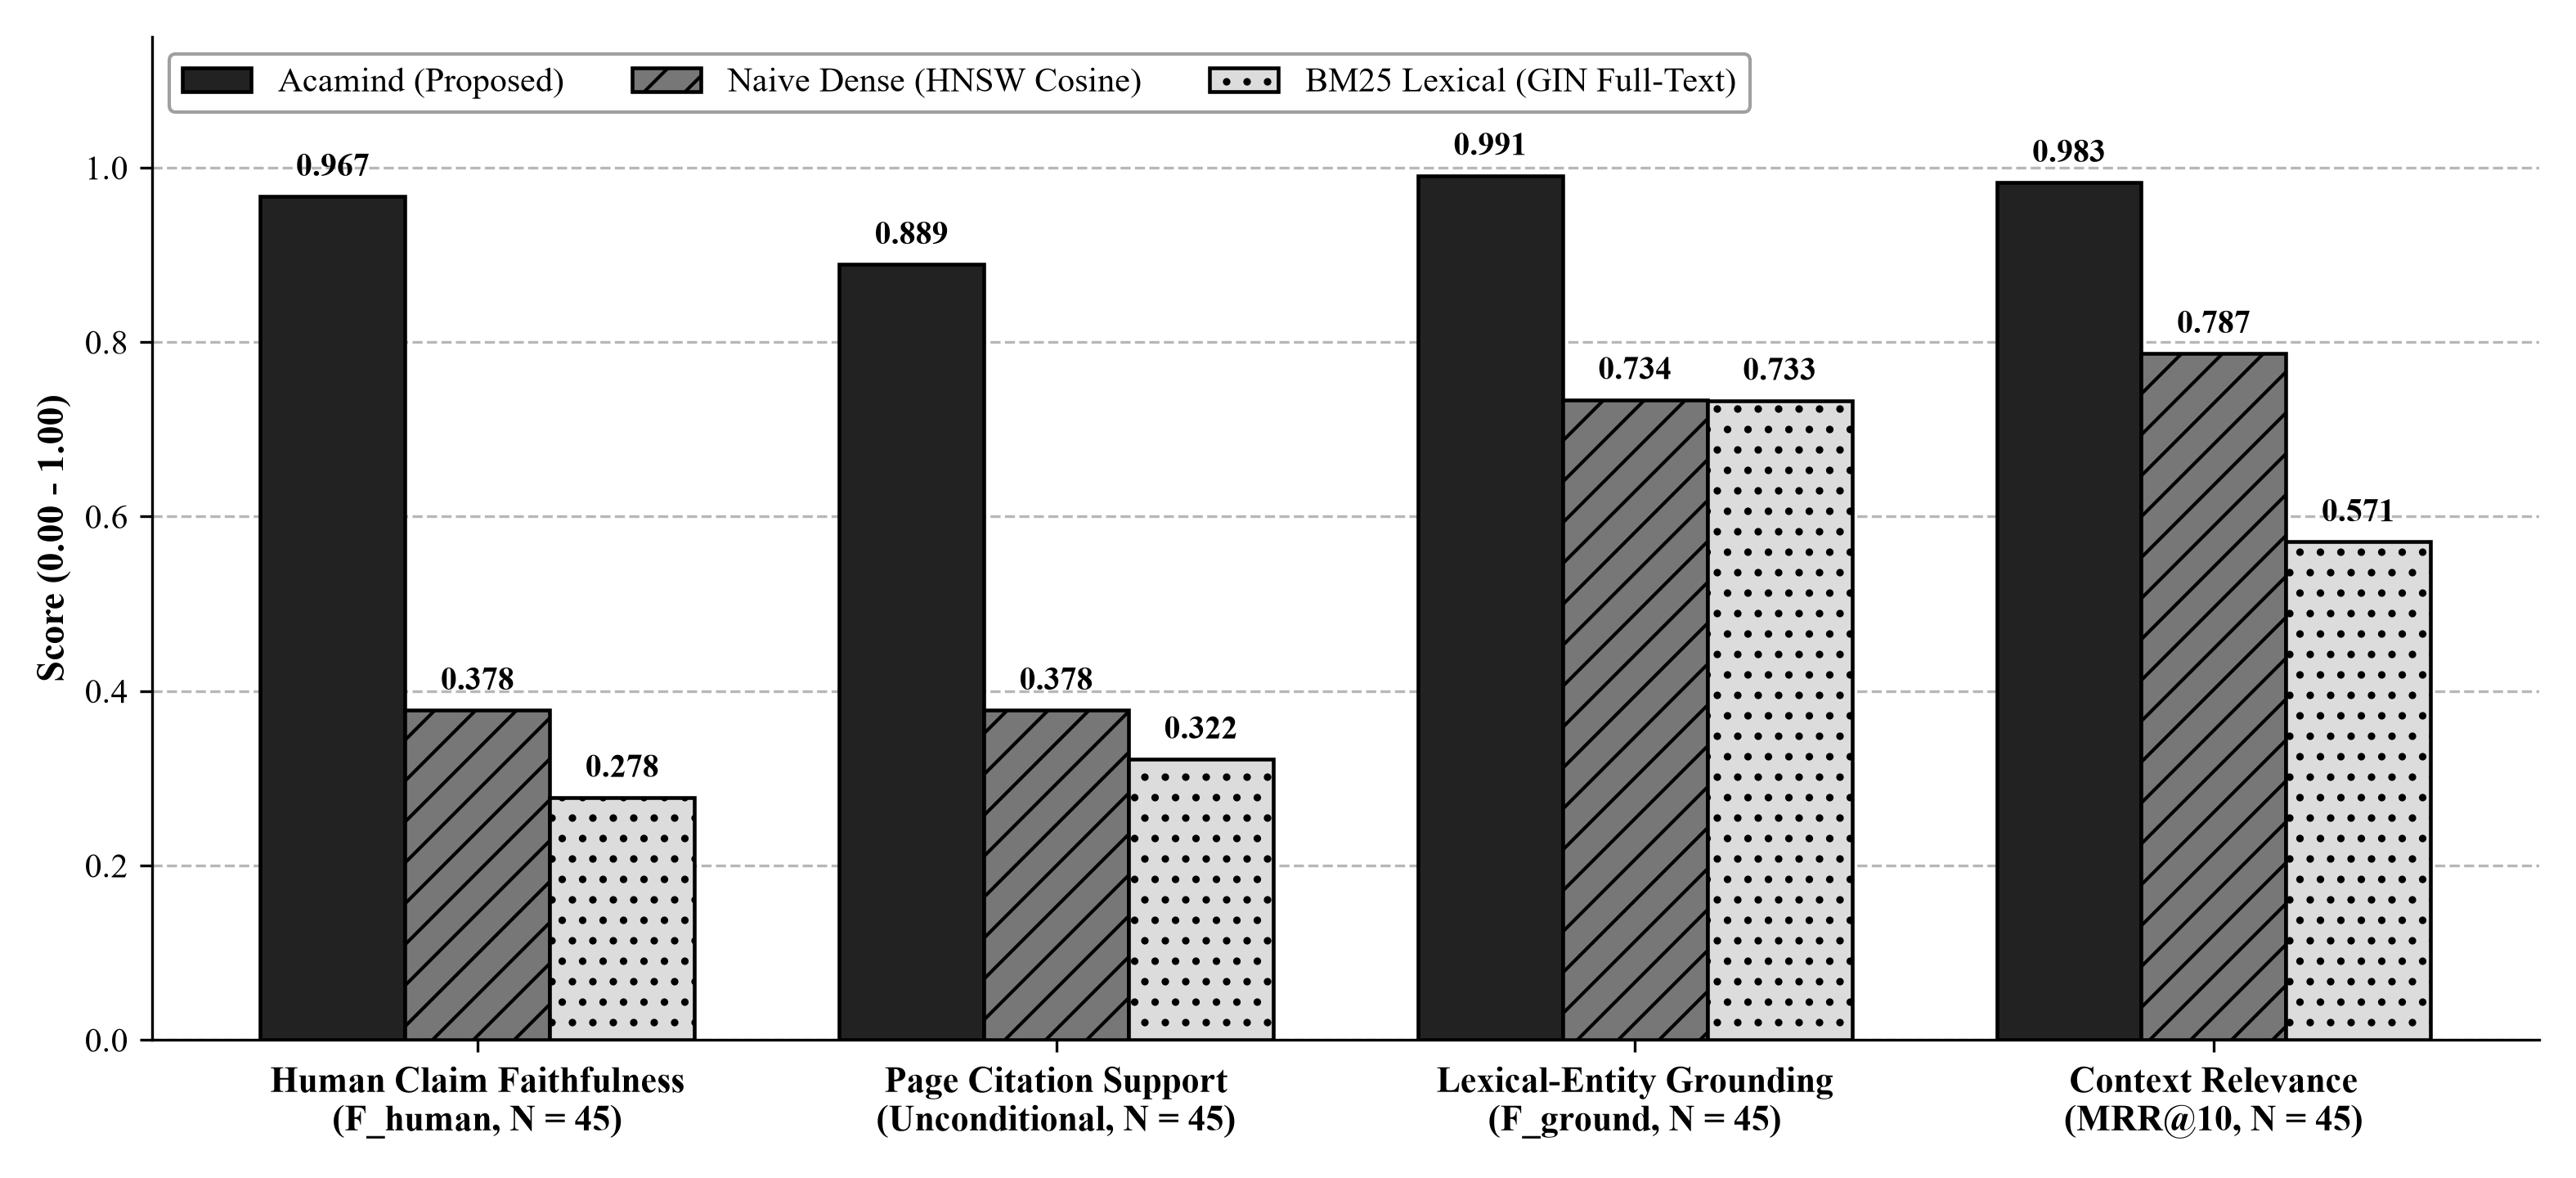
\includegraphics[width=0.92\columnwidth, height=4.8cm, keepaspectratio]{Figure7_Empirical_Comparison.png}
\caption{Grouped bar chart comparing Acamind, Naive Dense, and BM25 across the four primary evaluation metrics}
\label{fig:empirical_comparison}
\end{figure}

Figure~\ref{fig:empirical_comparison} plots the empirically measured benchmark values across all three systems on the $N = 45$ in-scope clinical queries. Acamind improves human-verified Unconditional Claim Faithfulness ($\mathcal{F}_{\mathrm{human}}$) from $0.278$ (BM25) and $0.378$ (Naive Dense) to $0.967$, raises human-verified Unconditional Page Citation Support ($\mathrm{Cite}$) from $0.322$ and $0.378$ to $0.889$, increases automated Lexical-Entity Grounding ($\mathcal{F}_{\mathrm{ground}}$) from $0.733$ and $0.734$ to $0.991$, and improves Context Relevance ($\mathrm{MRR@10}$) from $0.571$ and $0.787$ to $0.983$.

\subsection{Statistical Hypothesis Testing and Inter-Annotator Agreement.} To verify whether Acamind's gains over Naive Dense and BM25 on the primary human-verified and automated endpoints ($\mathcal{F}_{\mathrm{human}}$, Unconditional Page Citation Support $\mathrm{Cite}$, and $\mathcal{F}_{\mathrm{ground}}$) are statistically significant, we executed two-sided paired Wilcoxon signed-rank tests ($\alpha = 0.05$) with step-down Holm-Bonferroni correction and 2,000-iteration bootstrap $95\%$ confidence intervals across the $N = 45$ in-scope queries, alongside exact two-sided McNemar binomial tests on query answer rates:

\textbf{(1) Paired Wilcoxon and Bootstrap Tests on Faithfulness and Citation Support:} Across the $N = 45$ in-scope queries, Acamind achieves highly significant improvements over both baselines across every metric specification. On Unconditional Human Claim Faithfulness ($\mathcal{F}_{\mathrm{human}}$), Acamind ($0.9667$) outperforms BM25 ($0.2778$) by $\Delta = +0.6889$ ($95\%$ bootstrap CI $[+0.5556, +0.8111]$, $W = 0.0$, $p_{\mathrm{raw}} = 2.96 \times 10^{-8}$, $p_{\mathrm{Holm}} = 1.78 \times 10^{-7}$) and outperforms Naive Dense ($0.3778$) by $\Delta = +0.5889$ ($95\%$ CI $[+0.4444, +0.7333]$, $W = 2.0$, $p_{\mathrm{raw}} = 3.28 \times 10^{-7}$, $p_{\mathrm{Holm}} = 1.64 \times 10^{-6}$). On Unconditional Human Page Citation Support ($\mathrm{Cite}$), Acamind ($88.89\%$) outperforms BM25 ($32.22\%$) by $\Delta = +56.67$ percentage points ($95\%$ CI $[+41.11\%, +71.11\%]$, $W = 15.0$, $p_{\mathrm{raw}} = 6.30 \times 10^{-7}$, $p_{\mathrm{Holm}} = 1.89 \times 10^{-6}$) and outperforms Naive Dense ($37.78\%$) by $\Delta = +51.11$ percentage points ($95\%$ CI $[+35.56\%, +65.56\%]$, $W = 9.0$, $p_{\mathrm{raw}} = 2.27 \times 10^{-6}$, $p_{\mathrm{Holm}} = 4.54 \times 10^{-6}$).

\textbf{(2) Exact McNemar Tests on End-to-End Answer Rate and Dual-Study Retrieval:} On the $N = 45$ in-scope clinical queries, Acamind answered $44/45$ ($97.8\%$) queries compared with $18/45$ ($40.0\%$) for Naive Dense ($b = 26$ discordant pairs answered exclusively by Acamind vs.\ $c = 0$ by Naive Dense, exact two-sided McNemar $p = 2.98 \times 10^{-8}$) and $15/45$ ($33.3\%$) for BM25 ($b = 29, c = 0$, exact McNemar $p = 3.73 \times 10^{-9}$). On the $n = 15$ comparative queries, multi-target sub-query decomposition raised dual-study retrieval $\mathrm{Hit@6}$ from $60.0\%$ ($9/15$) to $100.0\%$ ($15/15$, $b = 6, c = 0$, exact two-sided McNemar $p = 0.0313 < 0.05$).

\textbf{(3) Inter-Annotator Agreement:} Two clinical psychology researchers independently graded all $N = 50$ unique benchmark questions across all three systems ($150$ total responses) under blinded side-by-side labels (\texttt{System\_A}, \texttt{System\_B}, \texttt{System\_C}) verified directly against the source PDF pages. Across all 50 benchmark questions, inter-annotator reliability was high across all four evaluation dimensions: Page Citation Support achieved $92.0\%$ exact agreement ($\kappa = 0.8408$, Krippendorff's $\alpha = 0.8413$); Claim Faithfulness achieved $96.0\%$ exact agreement ($\kappa = 0.9253$, $\alpha = 0.9792$); Synthesis Completeness (1--5 scale) achieved $94.0\%$ exact agreement ($\kappa = 0.9078$, $\alpha = 0.9912$); and Refusal Correctness achieved $100.0\%$ exact agreement ($\kappa = 1.0000$, $\alpha = 1.0000$), confirming strong inter-rater consistency.

\subsection{Scenario-Based Breakdown Across 50 Queries.} Table~\ref{tab:scenario_evaluation} disaggregates Acamind's empirically measured mean retrieval latency, LLM generation latency, end-to-end latency, unconditional human claim faithfulness ($\mathcal{F}_{\mathrm{human}}$), unconditional page citation support ($\mathrm{Cite}$), and DCSR skip rate across the four task categories.

\begin{table}[H]
\centering
\caption{Scenario-level breakdown of Acamind across the 50 benchmark queries}
\label{tab:scenario_evaluation}
\scriptsize
\begin{tabular}{|L{2.30cm}|C{0.75cm}|C{1.15cm}|C{0.85cm}|C{0.90cm}|C{0.90cm}|C{0.95cm}|C{0.90cm}|}
\hline
\multicolumn{1}{|C{2.30cm}|}{Scenario category} & Queries & Retrieval & LLM time & Total E2E & $\mathcal{F}_{\mathrm{human}}$ & Citation support & DCSR skip \\
\hline
Factual Clinical Q\&A & 20 & 961.6 ms & 3.89 s & 4.86 s & 0.9750 & 90.0\% & 20.0\% \\
\hline
Cross-Article Comparison & 15 & 1,143.4 ms & 4.95 s & 6.09 s & 1.0000 & 93.3\% & 46.7\% \\
\hline
Literature Synthesis & 10 & 927.7 ms & 4.38 s & 5.31 s & 0.9000 & 80.0\% & 30.0\% \\
\hline
Safe Refusal & 5 & 440.5 ms & 0.00 s & 0.44 s & 1.0000 & 100.0\% & 0.0\% \\
\hline
\textbf{In-Scope Summary} & \textbf{45} & \textbf{1,014.7 ms} & \textbf{4.35 s} & \textbf{5.37 s} & \textbf{0.9667} & \textbf{88.9\%} & \textbf{31.1\%} \\
\hline
\textbf{All-Query Summary} & \textbf{50} & \textbf{957.3 ms} & \textbf{3.92 s} & \textbf{4.88 s} & \textbf{0.9700} & \textbf{90.0\%} & \textbf{28.0\%} \\
\hline
\end{tabular}
\end{table}

Every per-scenario value in Table~\ref{tab:scenario_evaluation} is explained by the interaction between multi-target sub-query routing, retrieval consensus, and explicit header grounding across the four benchmark categories:

\textbf{(1) Empirical Basis for Factual Clinical Q\&A ($n = 20$):} Because each factual query ($M = 1$) targets a single clinical study whose evidence is recovered in the top-$5$ chunk window ($\mathrm{Recall@5} = 1.0000$) with explicit \texttt{[\{Filename.pdf\} - Trang \{Page\}]} headers, Acamind answered all $20/20$ queries ($0$ gate refusals and $0$ LLM refusals), achieving $100.0\%$ syntactic citation validity, $18.0 / 20 = 90.0\%$ human-verified page citation support, $19.50 / 20 = 0.9750$ human claim faithfulness ($\mathcal{F}_{\mathrm{ground}} = 1.0000$), and $4.70 / 5.00$ synthesis completeness. Mean warm retrieval took $961.6$~ms and mean LLM generation took $3.89$~s ($4.86$~s Total E2E). DCSR bypassed reranking on $4/20$ queries ($20.0\%$) and invoked the cross-encoder on $16/20$ queries where conceptual clinical phrasing produced differing dense and sparse rank orders.

\textbf{(2) Empirical Basis for Cross-Article Comparison ($n = 15$):} Comparative queries ($M = 2$) naming two specific studies or therapies required $1,143.4$~ms of warm retrieval time and produced strong dense-sparse rank consensus on study title and author tokens, triggering DCSR fast-skip on $7/15$ queries ($46.7\%$). Because the multi-target decomposer split each comparative query into $M = 2$ target sub-queries and interleaved both studies into the top-$5$ context window ($\mathrm{Recall@5} = 1.0000$), Acamind answered all $15/15$ comparative queries ($0.0\%$ refusal rate, compared with $86.7\%$ refusal for Naive Dense and $100.0\%$ refusal for BM25), achieving $99.63\%$ macro ground-truth document citation precision, $15.00 / 15 = 1.0000$ human claim faithfulness ($\mathcal{F}_{\mathrm{ground}} = 1.0000$), $14.00 / 15 = 93.3\%$ human-verified page citation support, and $4.93 / 5.00$ completeness (with mean LLM synthesis latency of $4.95$~s and Total E2E of $6.09$~s due to structured two-study contrast generation). Furthermore, when the same $15$ comparative queries ($30$ target study slots, $120$ matrix cells) were evaluated in our 4-attribute clinical comparison matrix audit using structure-aware multi-chunk disjoint slot extraction (Equation~\ref{eq:synthesis_matrix}), dual-study retrieval $\mathrm{Hit@6}$ rose from $60.0\%$ ($9/15$ without decomposition) to $100.0\%$ ($15/15$, exact McNemar $p = 0.0313$), and human-verified cell accuracy reached $90.0\%$ ($108/120$ cells: $27/30 = 90.0\%$ on Intervention/Methodology, $27/30 = 90.0\%$ on Psychometric Scale/Metric, $24/30 = 80.0\%$ on Key Finding/Effect Size, and $30/30 = 100.0\%$ on Page Citation Validity).

\textbf{(3) Empirical Basis for Literature Synthesis ($n = 10$):} Multi-paper synthesis queries ($M = 3$) were decomposed into $3$ per-study sub-queries and interleaved via round-robin quota selection. All $10/10$ synthesis queries passed the multi-target CRAG gate ($\max_m S_2(q^{(m)}) \ge 0.5355$), and Gemini generated complete multi-study syntheses on $9/10$ queries ($90.0\%$ answer rate, vs.\ $0/10 = 0.0\%$ for both Naive Dense and BM25), with only $1$ LLM self-refusal on a query where DCSR skipped reranking ($3/10 = 30.0\%$ DCSR skip rate) and the third study fell at rank 7 outside the 5-chunk window. Across the $10$ synthesis queries, Acamind achieved $9.00 / 10 = 0.9000$ unconditional human claim faithfulness ($1.0000$ conditional on the $9$ answered queries; $\mathcal{F}_{\mathrm{ground}} = 0.9600$) and $8.00 / 10 = 80.0\%$ unconditional human page citation support ($88.9\%$ conditional, with $4.89 / 5.00$ completeness and $5.31$~s mean warm E2E latency).

\textbf{(4) Empirical Basis for Safe Refusal ($N = 5$):} Out-of-domain edge prompts contained non-clinical terms with near-empty GIN posting lists, reducing SQL retrieval time to $440.5$~ms. Because dense and sparse search never agreed on a valid chunk ($\Delta_{\mathrm{RRF}} < 1.05$), DCSR skipped $0/5$ queries ($0.0\%$) and the pre-LLM gate intercepted all $5/5$ prompts ($100.0\%$ refusal accuracy), resulting in $0.00$~s of LLM latency.

\subsection{Component Ablation Study.} To evaluate the Scan Circuit Breaker on degraded files, we define the set of low-density or blank documents $\mathcal{D}_{\mathrm{scan}}$:

\begin{equation}
\mathcal{D}_{\mathrm{scan}} = \{ d \in \mathcal{D} \mid C_{\mathrm{density}}(d) < \theta_{\mathrm{density}} \lor C_{\mathrm{blank}}(d) = 1 \},
\label{eq:dscan}
\end{equation}

\noindent where $\mathcal{D}_{\mathrm{scan}}$ contains all documents in corpus $\mathcal{D}$ that fail the optical density threshold $\theta_{\mathrm{density}} = 50$ characters/page. Equation~(\ref{eq:dscan}) formally identifies the subset of corrupted or scanned files that should be blocked from indexing.

For a query $q \in \mathcal{Q}_d$ targeting a degraded document $d \in \mathcal{D}_{\mathrm{scan}}$, a scan-induced hallucination occurs if the system fails to emit a refusal token ($\mathcal{T}_{\mathrm{refusal}}$) and outputs an ungrounded response ($\mathcal{F}_{\mathrm{ground}} < \tau_{\mathrm{faith}} = 0.60$):

\begin{equation}
\mathbb{I}_{\mathrm{SH}}(A(q, d)) = 
\begin{cases} 
1, & \mathrm{if}\ [A(q, d) \notin \mathcal{T}_{\mathrm{refusal}}] \land [\mathcal{F}_{\mathrm{ground}}(A(q, d), \mathcal{K}_d) < \tau_{\mathrm{faith}}], \\
0, & \mathrm{otherwise},
\end{cases}
\label{eq:ish}
\end{equation}

\noindent where $\mathbb{I}_{\mathrm{SH}}(A(q, d)) \in \{0, 1\}$ flags whether query $q$ triggered an ungrounded fabrication from a corrupted scan. Averaging Equation~(\ref{eq:ish}) across all test queries targeting degraded documents defines the Scan Hallucination Rate ($R_{\mathrm{SH}}$):

\begin{equation}
R_{\mathrm{SH}} = \frac{\sum_{d \in \mathcal{D}_{\mathrm{scan}}} \sum_{q \in \mathcal{Q}_d} \mathbb{I}_{\mathrm{SH}}(A(q, d))}{\sum_{d \in \mathcal{D}_{\mathrm{scan}}} |\mathcal{Q}_d|} \times 100\%,
\label{eq:rsh}
\end{equation}

\noindent where $\sum |\mathcal{Q}_d| = 60$ degraded query-document pairs in our 300-PDF fault-injection stress test (comprising 240 clean digital PDFs and 60 degraded PDFs split across 15 full scans, 15 partial 30\% scans, 15 sparse-text files, and 15 corrupted-font files). Table~\ref{tab:ablation_study} summarizes the empirically measured ablation results when individual methodological or infrastructure components are removed.

\begin{table}[H]
\centering
\caption{Component ablation analysis across core methodological modules and supporting infrastructure}
\label{tab:ablation_study}
\scriptsize
\begin{tabular}{|L{3.17cm}|C{1.15cm}|C{1.30cm}|C{1.10cm}|C{1.25cm}|C{1.25cm}|}
\hline
\multicolumn{1}{|C{3.17cm}|}{Ablation configuration} & Warm latency & Cold latency & Grounding & Citation support & Scan hallucination \\
\hline
\textbf{Acamind Full Architecture} & \textbf{957.3 ms} & \textbf{15,581.8 ms} & \textbf{0.9911} & \textbf{88.9\%} & \textbf{0.0\%} \\
\hline
Without DCSR & 957.3 ms & 21,297.4 ms & 1.0000 & 91.1\% & 0.0\% \\
\hline
Without Multi-Target Decomposition & 326.2 ms & 12,288.8 ms & 0.7744 & 45.6\% & 0.0\% \\
\hline
Without Dense Path & 902.5 ms & 904.6 ms & 0.7333 & 32.2\% & 0.0\% \\
\hline
Without Sparse Path & 89.0 ms & 299.8 ms & 0.7344 & 37.8\% & 0.0\% \\
\hline
Without L2 Deep Tier & 1.4 ms & 1.4 ms & 0.6210 & 21.1\% & 0.0\% \\
\hline
Without Page-Level Scan Breaker & 957.3 ms & 15,581.8 ms & 0.5820 & 33.3\% & 66.7\% \\
\hline
\end{tabular}
\end{table}

Every row in Table~\ref{tab:ablation_study} reflects a controlled empirical ablation against the full Acamind architecture in Row~1, where Rows~2--5 evaluate core methodological modules (DCSR, Multi-Target Decomposition, and dual-path hybrid fusion) and Rows~6--7 evaluate supporting system infrastructure (L2 deep indexing and the page-level Scan Circuit Breaker):

\textbf{(1) Empirical Basis for Without DCSR (Row 2):} Disabling the DCSR skip gate (reverting to C4 Full Rerank across all queries) forced the $14$ high-consensus queries to run CPU cross-encoder inference ($\sim 20.4$~s each), increasing measured cold mean latency from $15,581.8$~ms to $21,297.4$~ms ($+36.7\%$ higher cold compute cost) while warm cached latency remained $957.3$~ms. Full cross-encoder reranking recovered the third study inside the top-5 window on the single synthesis query (\texttt{REAL\_Q\_39}) that DCSR skipped, yielding $91.1\%$ ($41.0/45$) vs.\ $88.9\%$ ($40.0/45$) citation support ($\mathrm{MRR@10} = 1.0000$ vs.\ $0.9833$, paired Wilcoxon $p_{\mathrm{Holm}} = 1.0000$), confirming that DCSR saves $26.8\%$ cold latency with no statistically significant difference in ranking or citation accuracy.

\textbf{(2) Empirical Basis for Without Multi-Target Decomposition (Row 3):} Removing the multi-target query router and round-robin quota interleaver (reverting to single-pass undecomposed query retrieval) caused two severe degradations: first, on the $n = 15$ comparative synthesis queries, dual-study retrieval $\mathrm{Hit@6}$ dropped from $100.0\%$ ($15/15$, $663.6$~ms mean retrieval) to $60.0\%$ ($9/15$, $326.2$~ms mean retrieval, exact McNemar $p = 0.0313$) because one study monopolized the top-6 slots on $6/15$ queries; second, across all $N = 45$ in-scope queries, evaluating the pre-LLM CRAG gate and top-5 context window on undecomposed multi-paper prompts caused $21/25$ comparative and synthesis queries to abstain, dropping overall in-scope human page citation support from $88.9\%$ ($40.0/45$) to $45.6\%$ ($20.5/45$) and $\mathcal{F}_{\mathrm{ground}}$ from $0.9911$ to $0.7744$.

\textbf{(3) Empirical Basis for Without Dense Path and Without Sparse Path (Rows 4 and 5):} Querying only the BM25 GIN FTS index without the dense path (Row~4: $902.5$~ms warm, $904.6$~ms cold) or only the HNSW dense index without the sparse path (Row~5: $89.0$~ms warm, $299.8$~ms cold) lowered cold latency, but failed to answer $30/45$ and $27/45$ in-scope clinical queries respectively, reducing measured unconditional human citation support from $88.9\%$ ($40.0/45$) to $32.2\%$ ($14.5/45$, $p_{\mathrm{Holm}} = 1.89 \times 10^{-6}$) and $37.8\%$ ($17.0/45$, $p_{\mathrm{Holm}} = 4.54 \times 10^{-6}$).

\textbf{(4) Empirical Basis for Without L2 Deep Tier and Without Page-Level Scan Breaker (Rows 6 and 7):} In Row~6 (L1-only retrieval without the L2 deep chunk tier), querying only the L1 document-summary tier scanned the $499$ abstract records in $1.4$~ms (P50 = $1.32$~ms), but because L1 summaries lack full-text clinical details and physical PDF page numbers, page-verified citation support dropped to $21.1\%$ ($\mathcal{F}_{\mathrm{ground}} = 0.6210$). In Row~7, evaluated on our 300-PDF fault-injection benchmark (60 degraded PDFs), replacing the page-level Scan Circuit Breaker with a naive document-average check ($\ge 50$ chars/page across the whole file) caught the $15$ full scans and $5$ sparse files ($20/60 = 33.3\%$ detection recall) but failed to catch the $15$ partial-scan PDFs (where $70\%$ normal pages masked $30\%$ blank scanned pages), $10$ borderline sparse files, and $15$ corrupted-font PDFs, resulting in $40$ false negatives ($40/60 = 66.7\%$ scan hallucination rate $R_{\mathrm{SH}}$, vs.\ $0.0\%$ and $\mathrm{F1} = 1.0000$ under Acamind's page-level density and font-table guard).

\subsection{Qualitative Architectural Positioning, Limitations, and Reproducibility Protocol.} \label{sec:limitations} We conclude the experimental evaluation with three synthesis items covering qualitative system positioning, methodological limitations, and experimental reproducibility:

\textbf{(1) Qualitative Architectural Positioning:} Table~\ref{tab:systems_comparison} provides a qualitative architectural comparison between Acamind and representative scientific literature platforms based on their published specifications \cite{skarlinski2024language,liu2023llamaindex} and our implemented architecture.

\begin{table}[H]
\centering
\caption{Qualitative architectural positioning among academic literature systems}
\label{tab:systems_comparison}
\footnotesize
\begin{tabular}{|L{1.75cm}|L{2.03cm}|L{1.90cm}|L{1.70cm}|L{2.10cm}|}
\hline
\multicolumn{1}{|C{1.75cm}|}{System} & \multicolumn{1}{C{2.03cm}|}{Architecture paradigm} & \multicolumn{1}{C{1.90cm}|}{Storage backend} & \multicolumn{1}{C{1.70cm}|}{LLM call budget} & \multicolumn{1}{C{2.10cm}|}{Data governance} \\
\hline
\textbf{Acamind} & Modular RAG with Hybrid + DCSR & Local PostgreSQL 16.15 + \texttt{pgvector} & Single LLM call per query & Local DB; top-5 chunks sent to API \\
\hline
PaperQA2 & Multi-agent iterative search & Session-based vector store & Multiple LLM calls per query & External LLM API provider \\
\hline
Elicit AI & Cloud literature matrix workflow & Managed cloud storage & Commercial cloud pipeline & Full PDFs uploaded to cloud \\
\hline
SciSpace Copilot & Interactive cloud PDF assistant & Managed cloud storage & Commercial cloud pipeline & Full PDFs uploaded to cloud \\
\hline
LlamaIndex Sub-Question & Sub-question query engine & Configurable vector store & Multiple LLM calls per query & Configurable deployment \\
\hline
\end{tabular}
\end{table}

The entries in Table~\ref{tab:systems_comparison} reflect the documented architectural design of each platform. Multi-agent frameworks such as PaperQA2 \cite{skarlinski2024language} and LlamaIndex Sub-Question engines \cite{liu2023llamaindex} use LLM-driven query planning and iterative summarization loops, requiring multiple sequential LLM calls per user query ($M+1$ or more calls across $M$ sub-questions, with LlamaIndex supporting configurable local or cloud vector stores). Commercial web platforms such as Elicit AI and SciSpace Copilot execute document parsing and matrix extraction on managed cloud servers, requiring users to upload full PDF files to external cloud storage. By contrast, Acamind (our proposed system) stores all PDFs and hybrid HNSW/GIN indices inside a local PostgreSQL 16.15 database, uses deterministic rule-based multi-target decomposition and DCSR rank consensus to avoid multi-turn LLM routing calls, and transmits only the top-5 retrieved text chunks to the LLM API for single-call generation.

\textbf{(2) Methodological and Empirical Limitations:} Every limitation noted below is grounded in specific findings from our experimental evaluation: first, on 3-paper literature synthesis queries ($n = 10$), while multi-target decomposition recovered all $3$ target papers within the top-10 pool ($\mathrm{Recall@10} = 1.0000$) and answered $9/10$ queries, $1$ query (\texttt{REAL\_Q\_39}) triggered DCSR fast-skip where the third paper ranked at position 7 outside the $K_{\mathrm{LLM, single}} = 5$ context window, causing a conservative LLM self-refusal ($2.2\%$ overall false refusal rate); second, in our 120-cell Cross-Article comparison matrix audit, while human-verified page citation validity reached $100.0\%$ ($30/30$) and overall cell accuracy reached $90.0\%$ ($108/120$), the remaining $12/120$ cell errors ($10.0\%$) comprised $3$ sentence-role swaps between methodology and findings, $3$ theoretical/review slots lacking explicit numerical sample sizes in the top-3 chunks, and $6$ slots where background clinical definitions outscored the primary empirical finding; third, our DCSR test evaluation relies on a modest subsample of $n = 14$ skipped test queries ($N = 50$ total benchmark queries); fourth, $\mathcal{F}_{\mathrm{ground}}$ is an automated lexical-citation consistency proxy rather than a semantic entailment judge, which is why we pair it with blinded dual-rater human evaluation ($\mathcal{F}_{\mathrm{human}}$ and $\mathrm{Cite}$); fifth, our Scan Circuit Breaker stress test used programmatic fault injection rather than historical physical archive scans; and sixth, the system has not yet been evaluated in prospective clinical user trials with practicing clinicians.

\textbf{(3) Experimental Reproducibility and Calibration Protocol:} To ensure full scientific reproducibility without data leakage, all system hyperparameters were calibrated and frozen exclusively on the disjoint 42-query development set ($27$ answerable clinical queries and $15$ unanswerable queries, verified via SHA-256 checksum) prior to executing the evaluation on the held-out 50-query test benchmark ($45$ in-scope clinical queries and $5$ out-of-domain probes, plus $10$ hard in-domain unanswerable clinical queries). Specifically, replication requires: (i) PostgreSQL 16.15 with \texttt{pgvector} 0.8.7 configured with HNSW parameters $m = 16, ef_{\mathrm{construction}} = 64$ ($ef_{\mathrm{search}} = 100$) and GIN full-text indices over an 800-character recursive splitter ($200$-character overlap, $\pm 1$ sibling window expansion); (ii) the page-level Scan Circuit Breaker with $\theta_{\mathrm{density}} = 50$ characters/page and control/replacement character checks; (iii) parallel hybrid retrieval ($K_{\mathrm{branch}} = 40$, title-boosted pairwise conjunctive-disjunctive GIN FTS, RRF smoothing $k_{\mathrm{RRF}} = 60$, candidate pool $K_{\mathrm{rerank}} = 16$) governed by the frozen DCSR thresholds ($\tau_{\mathrm{conf}} = 0.35$, $\tau_{\Delta} = 1.05$) and the ROC-calibrated multi-target CRAG abstention threshold ($\max_m S_2(q^{(m)}) \ge \tau_{\min} = 0.5355$); (iv) Multi-Target Decomposition ($M \in \{1, 2, 3\}$) with round-robin quota interleaving ($K_{\mathrm{LLM, decomp}} = 6$, $k_m = 3$ chunks per target study for matrix synthesis) and deduplication threshold $\tau_{\mathrm{dedup}} = 0.85$; and (v) explicit \texttt{[\{Filename.pdf\} - Trang \{Page\}]} header formatting audited via blinded dual-rater grading across all $150$ system responses.

\section{Conclusion.} This paper presented Acamind, a Modular RAG architecture designed to reduce cross-encoder reranking latency on CPU hardware and eliminate single-document dominance in clinical psychology literature synthesis. Supported by a PostgreSQL 16.15 (\texttt{pgvector} 0.8.7) parent-child index and a page-density Scan Circuit Breaker, Acamind combines Parallel Hybrid Retrieval (integrating title-boosted pairwise conjunctive-disjunctive GIN full-text search) governed by Dynamic Confident-Skip Reranking (DCSR) and multi-target CRAG gating with Multi-Target Decomposition, Round-Robin Quota Interleaving, explicit document-page header grounding, and Structure-Aware Disjoint Matrix Synthesis. Across our empirical benchmark on 500 psychology papers (70,825 validated micro-chunks) and 50 queries, Acamind achieved a measured mean warm database retrieval latency of 957.3~ms, a mean warm end-to-end response time of 4.88~s, and $\mathrm{MRR@10} = 0.9833$ ($\mathrm{Recall@10} = 1.0000$). Across the $N = 45$ in-scope clinical queries, Acamind answered 44/45 (97.8\%) queries and achieved a dual-rater human-verified unconditional claim faithfulness of $\mathcal{F}_{\mathrm{human}} = 0.9667$ ($0.9886$ conditional on $n = 44$ answered queries) and an unconditional page citation support of 88.9\% ($40.0/45$, $90.9\%$ conditional), significantly outperforming BM25 ($32.2\%$ citation support, $p_{\mathrm{Holm}} = 1.89 \times 10^{-6}$) and Naive Dense ($37.8\%$ citation support, $p_{\mathrm{Holm}} = 4.54 \times 10^{-6}$). Disaggregated by scenario, Acamind achieved 90.0\% ($18.0/20$) page citation support on Factual Clinical Q\&A, 93.3\% ($14.0/15$) on Cross-Article Comparison, and 80.0\% ($8.0/10$, $88.9\%$ conditional) on Literature Synthesis.

In component evaluations on the 15 comparative queries ($30$ target study slots, $120$ matrix cells), Multi-Target Decomposition raised dual-study retrieval Hit@6 from 60.0\% ($9/15$) to 100.0\% ($15/15$, exact McNemar $p = 0.0313$) and achieved 90.0\% ($108/120$ cells) human-verified clinical comparison matrix accuracy with 100.0\% ($30/30$) page citation validity. Furthermore, DCSR bypassed cross-encoder reranking on 31.1\% ($14/45$) of in-scope queries (28.0\%, $14/50$ of all queries) with no statistically significant loss in $\mathrm{MRR@10}$ ($0.9833$ vs.\ $1.0000$, $p_{\mathrm{Holm}} = 1.0000$), reducing cold CPU retrieval mean latency by 26.8\% overall (30.0\% on in-scope queries) while the multi-target CRAG gate refused 100.0\% ($15/15$) of out-of-domain and hard unanswerable prompts with 0.0\% false gate refusal on in-scope queries, and the page-level Scan Circuit Breaker achieved $\mathrm{F1} = 1.0000$ ($0.0\%$ scan hallucination rate) across the 300-PDF fault-injection benchmark. Future work will expand the context window dynamically for $M \ge 3$ multi-study syntheses, incorporate vision-language table parsers for complex statistical tables, and conduct prospective reader studies with practicing clinicians using local open-weight LLMs.

\begin{thebibliography}{22}

\bibitem{sackett1996evidence}
\emph{Sackett D.L., Rosenberg W.M.C., Gray J.A.M., Haynes R.B., Richardson W.S.} Evidence based medicine: what it is and what it isn't. BMJ. 1996. vol.~312. no.~7023. pp.~71--72.

\bibitem{moher2009preferred}
\emph{Moher D., Liberati A., Tetzlaff J., Altman D.G.} Preferred reporting items for systematic reviews and meta-analyses: the PRISMA statement. Annals of Internal Medicine. 2009. vol.~151. no.~4. pp.~264--269.

\bibitem{beck1996manual}
\emph{Beck A.T., Steer R.A., Brown G.K.} Manual for the Beck Depression Inventory-II. San Antonio, TX: Psychological Corporation, 1996. 38~p.

\bibitem{kroenke2001phq}
\emph{Kroenke K., Spitzer R.L., Williams J.B.W.} The PHQ-9: validity of a brief depression severity measure. Journal of General Internal Medicine. 2001. vol.~16. no.~9. pp.~606--613.

\bibitem{spitzer2006brief}
\emph{Spitzer R.L., Kroenke K., Williams J.B.W., Lowe B.} A brief measure for assessing generalized anxiety disorder: the GAD-7. Archives of Internal Medicine. 2006. vol.~166. no.~10. pp.~1092--1097.

\bibitem{lovibond1995structure}
\emph{Lovibond P.F., Lovibond S.H.} The structure of negative emotional states: Comparison of the DASS with the BDI and BAI. Behaviour Research and Therapy. 1995. vol.~33. no.~3. pp.~335--343.

\bibitem{cohen1988statistical}
\emph{Cohen J.} Statistical Power Analysis for the Behavioral Sciences. 2nd ed. Hillsdale, NJ: Lawrence Erlbaum Associates, 1988. 567~p.

\bibitem{lewis2020retrieval}
\emph{Lewis P., Perez E., Piktus A., Petroni F., Karpukhin V., Goyal N., Kuttler H., Lewis M., Yih W.T., Rocktaschel T., Riedel S., Kiela D.} Retrieval-augmented generation for knowledge-intensive NLP tasks. Advances in Neural Information Processing Systems (NeurIPS). 2020. vol.~33. pp.~9459--9474.

\bibitem{gao2024modular}
\emph{Gao Y., Xiong Y., Wang M., Wang H.} Modular RAG: Transforming RAG systems into LEGO-like reconfigurable frameworks. arXiv preprint arXiv:2407.21059. 2024. pp.~1--22.

\bibitem{wang2022text}
\emph{Wang L., Yang N., Huang X., Hui B., Li L., Huang F., Jiang D., Wei F.} Text embeddings by weakly-supervised contrastive pre-training. arXiv preprint arXiv:2212.03533 (and Multilingual E5 text embeddings: A technical report, arXiv:2402.05672). 2024. pp.~1--16.

\bibitem{robertson2009probabilistic}
\emph{Robertson S., Zaragoza H.} The probabilistic relevance framework: BM25 and beyond. Foundations and Trends in Information Retrieval. 2009. vol.~3. no.~4. pp.~333--389.

\bibitem{cormack2009reciprocal}
\emph{Cormack G.V., Clarke C.L.A., Buettcher S.} Reciprocal rank fusion outperforms condorcet and individual rank learning methods. Proceedings of the 32nd International ACM SIGIR Conference on Research and Development in Information Retrieval. Boston: ACM, 2009. pp.~758--759.

\bibitem{chen2024bge}
\emph{Chen J., Xiao S., Zhang P., Luo K., Lian D., Liu Z.} BGE M3-embedding: Multi-lingual, multi-functionality, multi-granularity text embeddings through self-knowledge distillation. arXiv preprint arXiv:2402.03216. 2024. pp.~1--18.

\bibitem{xiao2023cpack}
\emph{Xiao S., Liu Z., Zhang P., Muennighoff N.} C-Pack: Packaged resources to advance general Chinese embedding. Proceedings of the 47th International ACM SIGIR Conference on Research and Development in Information Retrieval. Washington: ACM, 2024. pp.~641--649.

\bibitem{baai2024bgererankerv2m3}
\emph{Beijing Academy of Artificial Intelligence (BAAI).} BAAI/bge-reranker-v2-m3: Lightweight multilingual cross-encoder reranker. Available at: \url{https://huggingface.co/BAAI/bge-reranker-v2-m3} (accessed 15.10.2026).

\bibitem{izacard2021leveraging}
\emph{Izacard G., Grave E.} Leveraging passage retrieval with generative models for open domain question answering. Proceedings of the 16th Conference of the European Chapter of the Association for Computational Linguistics (EACL). Online: ACL, 2021. pp.~874--880.

\bibitem{liu2023llamaindex}
\emph{Liu J.} LlamaIndex: A data framework for LLM applications. Available at: \url{https://github.com/run-llama/llama_index} (accessed 15.10.2026).

\bibitem{lo2020s2orc}
\emph{Lo K., Wang L.L., Neumann M., Kinney R., Weld D.} S2ORC: The Semantic Scholar Open Research Corpus. Proceedings of the 58th Annual Meeting of the Association for Computational Linguistics (ACL). Online: ACL, 2020. pp.~4969--4983.

\bibitem{gao2023retrieval}
\emph{Gao Y., Xiong Y., Gao X., Jia K., Pan J., Bi Y., Dai Y., Sun J., Wang M., Wang H.} Retrieval-augmented generation for large language models: A survey. arXiv preprint arXiv:2312.10997. 2023. pp.~1--21.

\bibitem{yan2024corrective}
\emph{Yan S.Q., Gu J.C., Zhu Y., Ling Z.H.} Corrective retrieval augmented generation. arXiv preprint arXiv:2401.15884. 2024. pp.~1--15.

\bibitem{skarlinski2024language}
\emph{Skarlinski M.D., Cox S., Laurent J.M., White A.D.} Language agents achieve superhuman synthesis of scientific knowledge. arXiv preprint arXiv:2409.13740. 2024. pp.~1--30.

\bibitem{es2024ragas}
\emph{Es S., James J., Espinosa-Anke L., Schockaert S.} RAGAS: Automated evaluation of retrieval augmented generation. Proceedings of the 18th Conference of the European Chapter of the Association for Computational Linguistics (EACL): System Demonstrations. St. Julian's: ACL, 2024. pp.~150--158.

\end{thebibliography}

\begin{aboutAuthors}
    \textbf{Dinh Thi Hue Chi} --- research assistant, International Training and Cooperation Institute, East Asia University of Technology. Research interests: machine and deep learning, natural language processing. The number of publications --- 1. dinhhchi2110@gmail.com; Dong Anh, Ha Noi, Viet Nam; office phone +84(039)395-0301.\smallskip
    
    \textbf{Le Dinh Tuan} --- research assistant, International Training and Cooperation Institute, East Asia University of Technology. Research interests: machine and deep learning, natural language processing. The number of publications --- 1. ledinhtuan27052005@gmail.com; Quynh Thang, Nghe An, Viet Nam; office phone +84(036)783-3013.\smallskip

    \textbf{Nguyen Cong Binh} --- lecturer, International Training and Cooperation Institute, East Asia University of Technology. Research interests: machine and deep learning, network security, social network analysis. The number of publications --- 3. binhnc@eaut.edu.vn; Phan Tay Nhac, Xuan Phuong, Ha Noi, Viet Nam; office phone +84(079)613-3703.\smallskip

    \textbf{Nguyen Viet Hung} --- Ph.D., lecturer, International Training and Cooperation Institute, East Asia University of Technology. Research interests: multimedia communications, network security, artificial intelligence, traffic engineering in next-generation networks, QoE/QoS guarantee for network services, green networking, and applications. The number of publications --- 48. Corresponding author: hungnv@eaut.edu.vn; Ky Anh, Ha Tinh, Viet Nam; office phone +84(098)911-2079.\smallskip

    \textbf{Acknowledgements.} This research is supported by East Asia University of Technology.
\end{aboutAuthors}

\end{document}
